\chapter{Epicycle Sets and Deferent Sphere Sets}
\label{chap:dyn_epicycle}
\markboth{Epicycle Sets and Deferent Sphere Sets}{Epicycle Sets and Deferent Sphere Sets}

\begin{remark}[Positioning of this chapter]\label{rem:dyn_chapter_positioning}
This chapter follows directly on the `Vector Analysis' chapter: it generalises the static three-group projection model established there into a dynamic model, and supplies the three classes of object that were still missing---single-group dynamics, the quaternion single-sphere group and the rotating sphere group. The whole chapter follows a uniform two-step structure:
\[
\textbf{Composition} \;\longrightarrow\; \textbf{Projection} \;\longrightarrow\; \textbf{Observation result}.
\]
\textbf{Convention}: every model in this chapter adopts the order `compose first, project afterwards'. That is, the time group and the space group are first combined into a composite object (in the complex case the sum $T+S$, in the quaternion case the sum $q_T+q_S$), and this composite object is then projected onto the observer group. The observer itself may vary with time, and may also rotate independently according to its own epicycle.

\textbf{Guide to the seven themes}: Translation---the dynamic adjustment of the observer vector and frequency translation; Scaling---the weight introduced by the observer's modulus and the slow amplitude modulation of the envelope; Rotation---the independent rotation of the three planes and of the three episphere groups; Balance---the linearity of composition and projection; Symmetry---the symmetry and commutativity of projection; Closure---the invariants of synchronous rotation; Period---the instantaneous frequency, the beat frequency and the envelope period of the dynamic projection.
\end{remark}

\begin{figure}[htbp]
\centering
\begin{tikzpicture}[
  font=\small,
  box/.style={draw, rounded corners, fill=blue!8, minimum width=2.6cm, minimum height=0.8cm, align=center},
  sub/.style={draw, rounded corners, fill=green!10, minimum width=2.4cm, minimum height=0.7cm, align=center, font=\footnotesize},
  arr/.style={->, thick, >=stealth}
]
  \node[box] (pre) {Preliminary four series\\amplitude/frequency/phase/period};
  \node[box, right=0.9cm of pre] (single) {Single-group dynamic epicycle\\$\mathcal E(t)$};
  \node[box, right=0.9cm of single] (triple) {Three-group dynamic epicycle\\$T,S,O$};
  \node[box, right=0.9cm of triple] (rotating) {Rotating three planes\\rotating by the internal epicycles};
  \node[sub, below=1.0cm of pre] (quat) {Quaternion single-sphere group\\$q_T,q_S,q_O$};
  \node[sub, below=1.0cm of single] (rotquat) {Rotating three-sphere groups\\$r_jq_jr_j^{-1}$};
  \node[sub, below=1.0cm of triple] (unified) {Unified observer projection\\$\Pi_O(X)=\operatorname{Re}[X\overline O]$};
  \node[sub, below=1.0cm of rotating] (observer) {Observer functor\\adjunction $\Pi_O\dashv\Pi_O^*$};
  \node[sub, below=1.0cm of quat] (info) {Projection information compression\\DPI and rate distortion};

  \node[box, fill=orange!12] (extra) at ($(pre)!0.5!(rotating) + (0,-5.0)$)
       {Discrete unitary dynamic projection + scale-dependent sampling + information loss with distance};
  \draw[arr] (pre) -- (single);
  \draw[arr] (single) -- (triple);
  \draw[arr] (triple) -- (rotating);
  \draw[arr] (pre) -- (quat);
  \draw[arr] (single) -- (rotquat);
  \draw[arr] (triple) -- (unified);
  \draw[arr] (rotating) -- (observer);
  \draw[arr] (quat) -- (info);
  \draw[arr] (rotquat) -- (extra);
  \draw[arr] (unified) -- (extra);
  \draw[arr] (observer) -- (extra);
  \draw[arr] (info) -- (extra);
\end{tikzpicture}
\caption{Overview of the structure of this chapter: starting from the preliminary four series, the single-group dynamic epicycle, the three-group dynamic epicycle, the rotating three planes, the quaternion single-sphere group, the rotating three-sphere groups, the unified observer projection framework, the observer functor and projection information compression are established in turn, finally converging on discrete unitary dynamic projection, scale-dependent sampling and information loss with distance.}
\label{fig:dyn_overview}
\end{figure}

\section{Preliminaries: the four series and the definition of epicycles}
\label{sec:dyn_prerequisites}

This section recapitulates the amplitude series, frequency series, phase series and period series established in the `Series and Convolution' chapter, and on this basis defines the basic objects of this chapter---epicycles and epispheres. The content of this section is a citation and recombination of the preceding chapters; it introduces no new mathematical assertions.

\subsection{Amplitude series}

\begin{definition}[Amplitude series (recap)]\label{def:dyn_amplitude_series}
Let the amplitude sequence $\{A_k\}_{k\in\mathbb Z}$ satisfy $A_k\ge 0$ and $\sum_k A_k<\infty$. The formal series
\[
\mathcal A_f(t)=\sum_{k\in\mathbb Z}A_k e^{ikt}
\]
is called the \textbf{amplitude series} (its real form is $\sum_k A_k\cos(kt)$, requiring $A_{-k}=A_k$). The amplitude series retains only the amplitude information, discarding the phase and the frequency-lattice structure.

\textbf{Prerequisite}: absolute summability $\sum_k A_k<\infty$ guarantees uniform convergence (`Series and Convolution' chapter \cref{lem:absolute-summability-convergence}).
\end{definition}

\begin{proposition}[Bohr mean coefficient formula for the amplitude series (recap)]\label{prop:dyn_amplitude_coefficient}
Let $\mathcal A_f(t)=\sum_k A_k e^{ikt}$ converge uniformly and absolutely. Then for every $n\in\mathbb Z$,
\[
A_n=M\{\mathcal A_f(t)e^{-int}\}=\lim_{T\to\infty}\frac{1}{2T}\int_{-T}^{T}\mathcal A_f(t)e^{-int}\,dt.
\]
That is, the amplitude $A_n$ can be extracted uniquely by the Bohr mean.
\end{proposition}

\begin{proof}
By absolute summability the Bohr mean may be interchanged with the sum:
\[
M\{\mathcal A_f(t)e^{-int}\}=\sum_k A_k M\{e^{i(k-n)t}\}.
\]
By the orthogonality of the exponential basis (`Series and Convolution' chapter \cref{lem:amplitude_exponential_mean}), $M\{e^{i(k-n)t}\}=\delta_{kn}$, so only the term $k=n$ survives, giving $A_n$.
\end{proof}

\subsection{Frequency series}

\begin{definition}[Frequency series (recap)]\label{def:dyn_frequency_series}
Let $f$ have fundamental period $T$, with frequency lattice $\omega_n=2\pi n/T$. The formal series
\[
\mathcal F_f(s)=\sum_{n\in\mathbb Z}\omega_n s^n=\frac{2\pi}{T}\sum_{n\in\mathbb Z}n s^n
\]
is called the \textbf{frequency series}. The frequency series retains only the frequency lattice, discarding amplitude and phase.
\end{definition}

\begin{proposition}[Frequency series and period scaling (recap)]\label{prop:dyn_frequency_scaling}
If $f_\lambda(t):=f(t/\lambda)$ ($\lambda>0$), then the frequency series scales as $\mathcal F_{f_\lambda}(s)=\frac{1}{\lambda}\mathcal F_f(s)$.
\end{proposition}

\begin{proof}
$f_\lambda$ has period $\lambda T$, hence its frequencies are $\omega_n^{(\lambda)}=2\pi n/(\lambda T)=\omega_n/\lambda$; substituting into \cref{def:dyn_frequency_series} gives the result.
\end{proof}

\subsection{Phase series}

\begin{definition}[Phase series (recap)]\label{def:dyn_phase_series}
Let $\{\phi_k\}_{k\in\mathbb Z}$ be a phase sequence. The formal series
\[
\mathcal P_f(t)=\sum_{k\in\mathbb Z}e^{i(kt+\phi_k)}
\]
is called the \textbf{phase series}. The phase series retains only the phase, discarding amplitude and frequency-lattice structure.
\end{definition}

\begin{proposition}[Phase series and time translation (recap)]\label{prop:dyn_phase_translation}
The time translation $f_\tau(t):=f(t-\tau)$ rotates every term of the phase series by $-k\tau$:
\[
\mathcal P_{f_\tau}(t)=\sum_k e^{i(kt+\phi_k-k\tau)}.
\]
\end{proposition}

\begin{proof}
Substituting $t\mapsto t-\tau$: $e^{i(k(t-\tau)+\phi_k)}=e^{i(kt+\phi_k-k\tau)}$; summing gives the result.
\end{proof}

\subsection{Period series}

\begin{definition}[Period series (recap)]\label{def:dyn_periodic_series}
Let $P$ be an index set of period classes, $T_p>0$, and let the quadruple $(A_{p,n},\omega_{p,n},\phi_{p,n},T_p)$ satisfy $\omega_{p,n}=2\pi n/T_p$. The series
\[
f(t)=\sum_{p\in P}\sum_{n\in\mathbb Z}A_{p,n}e^{i(\omega_{p,n}t+\phi_{p,n})}
\]
is called the \textbf{period series}. The period series takes the period $T_p$ as its primary index; within each period layer the amplitude series supplies $A_{p,n}$, the phase series supplies $e^{i\phi_{p,n}}$, and the frequency series supplies $\omega_{p,n}$.
\end{definition}

\begin{proposition}[The period series synthesises the four series (recap)]\label{prop:dyn_periodic_synthesis}
The period series is synthesised from the four components amplitude, phase, frequency and period according to the period layer $p$. For a single period layer $P=\{T\}$ it degenerates to the Fourier series; taking the phase to be zero or the amplitude to be one further yields the amplitude series or the phase series respectively.
\end{proposition}

\begin{proof}
By Definition \ref{def:dyn_periodic_series}, for fixed $p$ the inner sum $\sum_n A_{p,n}e^{i(\omega_{p,n}t+\phi_{p,n})}$ is a standard Fourier series. Taking $P=\{T\}$ gives a single layer; taking $\phi_{p,n}\equiv0$ gives the amplitude series; taking $A_{p,n}\equiv1$ gives the phase series. Checking term by term gives the result.
\end{proof}

\subsection{Epicycles: periodic elements in the complex plane}

\begin{definition}[Epicycle]\label{def:dyn_epicycle}
Let $A>0$, $\omega\in\mathbb R$, $\phi\in[0,2\pi)$. The map
\[
\gamma_{A,\omega,\phi}:\mathbb R\to\mathbb C,\qquad
\gamma_{A,\omega,\phi}(t)=A e^{i(\omega t+\phi)}
\]
is called an \textbf{epicycle}. The three parameters are called the \textbf{radius} (amplitude), the \textbf{angular velocity} (frequency) and the \textbf{initial phase} respectively.

\textbf{Prerequisite}: $A>0$. If $A=0$, the epicycle degenerates to the zero map.
\end{definition}

\begin{figure}[htbp]
\centering
\begin{tikzpicture}[scale=2.0,>=stealth]
  \draw[->] (-2.0,0) -- (2.0,0) node[right]{$\Re$};
  \draw[->] (0,-2.0) -- (0,2.0) node[above]{$\Im$};

  \draw[thick,blue] (0,0) circle (1.4);
  \draw[->,thick,blue] (0,0) -- (1.4,0) node[midway,below,font=\footnotesize]{$A$};
  \filldraw[blue] (1.4,0) circle (2pt);

  \draw[->,thick,red] (0.6,0) arc (0:60:0.6);
  \node[red,font=\footnotesize,xshift=0.5cm] at (0.7,0.35) {$\omega t+\phi$};
  \draw[->,thick,blue] (1.4,0) arc (0:120:1.4);
  \node[blue,font=\footnotesize] at (1.0,1.5) {$\gamma_{A,\omega,\phi}(t)$};
  \node[font=\footnotesize] at (0,-2.4) {Epicycle in the complex plane};
\end{tikzpicture}
\caption{Epicycle: uniform circular motion in the complex plane with radius $A$, angular velocity $\omega$ and initial phase $\phi$.}
\label{fig:dyn_epicycle}
\end{figure}

\begin{definition}[Epicycle group]\label{def:dyn_epicycle_group_def}
Let $K\in\mathbb N^+$, $\{A_k\}_{k=1}^{K}\subset\mathbb R^+$, $\{\omega_k\}_{k=1}^{K}\subset\mathbb R$, $\{\phi_k\}_{k=1}^{K}\subset[0,2\pi)$. The finite sum
\[
\mathcal E(t)=\sum_{k=1}^{K}A_k e^{i(\omega_k t+\phi_k)}
\]
is called an \textbf{epicycle group}. The composite trajectory $\mathcal E(t)$ is a curve in the complex plane.

\textbf{Relation to the four series}: \cref{def:dyn_epicycle_group_def} is the concrete realisation of the period series on a single period layer under truncation to a finite series. Its amplitudes are given by the amplitude series ($\{A_k\}$), its phases by the phase series ($\{\phi_k\}$), its frequencies by the frequency series ($\{\omega_k\}$), and the common period $T=2\pi/\lvert\omega_0\rvert$ (with $\omega_0=\gcd\{\omega_k\ne0\}$ the fundamental frequency) by the period component.
\end{definition}

\begin{figure}[htbp]
\centering
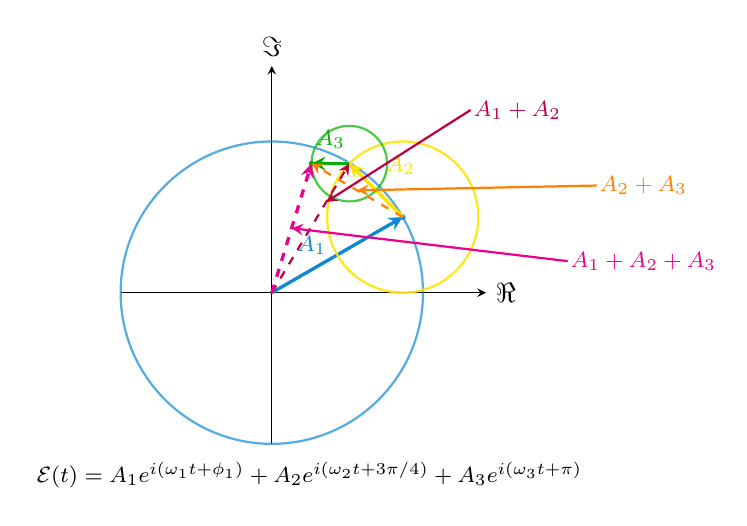
\begin{tikzpicture}[scale=1.6,>=stealth,
  lbl/.style={font=\footnotesize, inner sep=1pt}]

  \draw[->] (-1.2,0) -- (1.7,0) node[right]{$\Re$};
  \draw[->] (0,-1.2) -- (0,1.8) node[above]{$\Im$};

  \draw[thick,cyan!70!blue,opacity=0.7] (0,0) circle (1.2);
  \draw[->,very thick,cyan!70!blue] (0,0) -- (1.0392,0.6)
       node[lbl, pos=0.45, above left]{$A_1$};
  \filldraw[cyan!70!blue] (1.0392,0.6) circle (0.5pt);

  \draw[thick,yellow!85!orange,opacity=0.9] (1.0392,0.6) circle (0.6);
  \draw[->,very thick,yellow!85!orange] (1.0392,0.6) -- (0.6149,1.0243)
       node[lbl, pos=0.55, above right, xshift=3pt, yshift=3pt]{$A_2$};
  \filldraw[yellow!85!orange] (0.6149,1.0243) circle (0.5pt);

  \draw[thick,green!70!black,opacity=0.7] (0.6149,1.0243) circle (0.3);
  \draw[->,very thick,green!70!black] (0.6149,1.0243) -- (0.3149,1.0243)
       node[lbl, pos=0.5, above, yshift=4pt]{$A_3$};
  \filldraw[green!70!black] (0.3149,1.0243) circle (0.5pt);

  \draw[->,thick,purple,dashed]  (0,0)         -- (0.6149,1.0243);
  \draw[->,thick,orange,dashed]  (1.0392,0.6)  -- (0.3149,1.0243);
  \draw[->,very thick,magenta,dashed] (0,0)    -- (0.3149,1.0243);

  \node[lbl, purple]  (lbl12)  at (1.95, 1.45) {$A_1+A_2$};
  \draw[->, thick, purple]  (lbl12.west)  -- (0.43, 0.72);

  \node[lbl, orange]  (lbl23)  at ([xshift=1cm]1.95, 0.85) {$A_2+A_3$};
  \draw[->, thick, orange]  (lbl23.west)  -- (0.677, 0.812);

  \node[lbl, magenta] (lbl123) at ([xshift=1cm]1.95, 0.25) {$A_1+A_2+A_3$};
  \draw[->, thick, magenta] (lbl123.west) -- (0.157, 0.512);

  \node[font=\footnotesize] at (0.3,-1.45)
    {$\mathcal E(t)=A_1e^{i(\omega_1t+\phi_1)}+A_2e^{i(\omega_2t+3\pi/4)}+A_3e^{i(\omega_3t+\pi)}$};
\end{tikzpicture}
\caption{Epicycle group: the arm $A_1$ (cyan, length $r_1$) lies inside the circle $A_1$, the arm $A_2$ (yellow, length $r_2$, phase $135^\circ$) lies inside the circle $A_2$, and the arm $A_3$ (green, length $r_3$, phase $\pi$) lies inside the circle $A_3$; the endpoint of each arm is the centre of the next circle. The three composite vectors $A_1+A_2$ (purple dashed), $A_2+A_3$ (orange dashed) and $A_1+A_2+A_3$ (magenta dashed) are the instantaneous values of the composite trajectory at the various levels; their textual labels are placed outside on the right of the figure, with arrows of the same colour pointing to the corresponding dashed lines.}
\label{fig:dyn_epicycle_group}
\end{figure}

\begin{proposition}[Periodicity condition for the epicycle group]\label{prop:dyn_epicycle_period_condition}
Let $\mathcal E(t)=\sum_{k=1}^{K}A_k e^{i(\omega_k t+\phi_k)}$ with $A_k>0$ for all $k$. Then $\mathcal E$ is a periodic function if and only if all the $\omega_k$ generate a discrete subgroup. In that case write
\[
\omega_0:=\min\{\omega>0:\omega\in\textstyle\sum_k\mathbb{Z}\omega_k\}=\gcd\{\omega_k\ne0\},
\]
(that is, $\omega_k/\omega_0\in\mathbb Z$ for all $k$); then the least positive period is $2\pi/\lvert\omega_0\rvert$ (an integer fraction of it when $\omega_0\notin\Omega$); when all $\omega_k=0$ there is no least positive period.
\end{proposition}

\begin{proof}
\textbf{Sufficiency}. If $\omega_k=n_k\omega_0$ ($n_k\in\mathbb Z$), then
\[
\mathcal E(t+T)=\sum_k A_k e^{i(n_k\omega_0(t+2\pi/\omega_0)+\phi_k)}
=\sum_k A_k e^{i(n_k\omega_0 t+\phi_k+2\pi n_k)}
=\sum_k A_k e^{i(n_k\omega_0 t+\phi_k)}=\mathcal E(t).
\]

\textbf{Necessity}. If $\mathcal E$ has period $T>0$, then for each $k$, $e^{i\omega_k T}=1$, that is $\omega_k T\in 2\pi\mathbb Z$. Taking $\omega_0=2\pi/T$ gives $\omega_k/\omega_0=\omega_k T/(2\pi)\in\mathbb Z$. Hence all frequencies are integer multiples of $\omega_0$.
\end{proof}

\begin{remark}[Connection with the static model]\label{rem:dyn_epicycle_static_link}
\cref{def:dyn_epicycle_group_def} agrees, as a mathematical object, with the nested epicycle group established in the `Vector Analysis' chapter---both are finite sums of complex exponentials in the complex plane. What is new in this chapter is that the parameters of these epicycles are regarded as functions that may vary with time, and the resulting dynamic projection is studied.
\end{remark}

\subsection{Epispheres: periodic elements in quaternion space}

\begin{definition}[Episphere]\label{def:dyn_epicycle_ball}
Let $a>0$, let $\mathbf u$ be a unit pure imaginary quaternion ($\mathbf u^2=-1$), and let $\theta\in\mathbb R$. The map
\[
\beta_{a,\mathbf u,\theta}:\mathbb R\to\mathbb H,\qquad
\beta_{a,\mathbf u,\theta}(t)=a\,e^{\mathbf u\theta t}
\]
is called an \textbf{episphere}. Here $e^{\mathbf u\theta t}=\cos(\theta t)+\mathbf u\sin(\theta t)$ is the quaternion exponential.

The three parameters are called the \textbf{radius} ($a$), the \textbf{rotation axis} ($\mathbf u$) and the \textbf{angular velocity} ($\theta$) respectively.
\end{definition}

\begin{figure}[htbp]
\centering
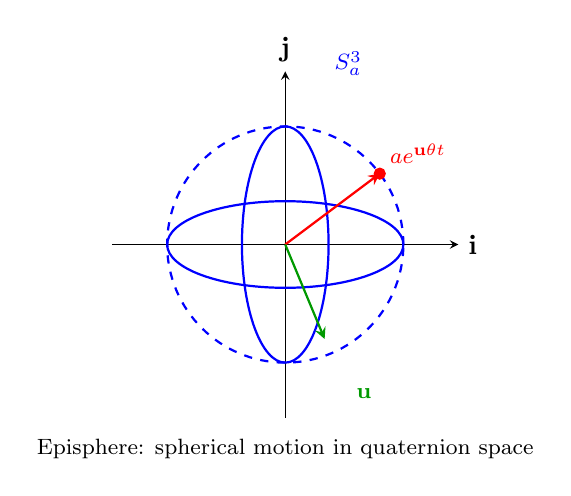
\begin{tikzpicture}[scale=1.0,>=stealth]
  \draw[->] (-2.2,0) -- (2.2,0) node[right]{$\mathbf i$};
  \draw[->] (0,-2.2) -- (0,2.2) node[above]{$\mathbf j$};

  \draw[thick,blue,dashed] (0,0) circle (1.5);
  \draw[thick,blue] (0,0) ellipse (1.5 and 0.55);
  \draw[thick,blue] (0,0) ellipse (0.55 and 1.5);

  \draw[->,thick,red] (0,0) -- (1.2,0.9) node[above right,font=\footnotesize]{$a e^{\mathbf u\theta t}$};
  \filldraw[red] (1.2,0.9) circle (2pt);

  \draw[->,thick,green!60!black] (0,0) -- (0.5,-1.2) node[below,font=\footnotesize,xshift=0.5cm,yshift=-0.5cm]{$\mathbf u$};

  \node[blue,font=\footnotesize,xshift=-1cm,yshift=1cm] at (1.8,1.3) {$S^3_a$};
  \node[font=\footnotesize] at (0,-2.6) {Episphere: spherical motion in quaternion space};
\end{tikzpicture}
\caption{Episphere: the orbit of radius $a$ in quaternion space lies on the three-dimensional sphere $S^3_a$.}
\label{fig:dyn_epicycle_ball}
\end{figure}

\begin{definition}[Episphere group]\label{def:dyn_epicycle_ball_group_def}
Let $K\in\mathbb N^+$, $a_k>0$, let $\mathbf u_k$ be a unit pure imaginary quaternion, and let $\theta_k\in\mathbb R$. The finite sum
\[
q(t)=\sum_{k=1}^{K}a_k e^{\mathbf u_k\theta_k t}
\]
is called an \textbf{episphere group}.
\end{definition}

\begin{figure}[htbp]
\centering
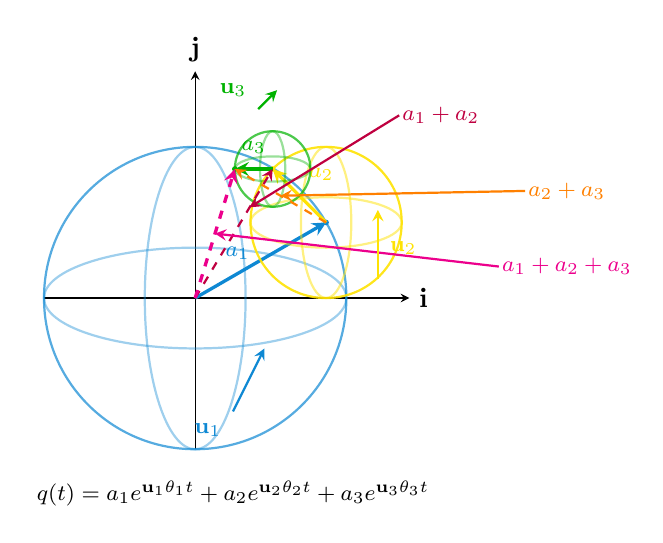
\begin{tikzpicture}[scale=1.6,>=stealth,
  lbl/.style={font=\footnotesize, inner sep=1pt}]

  \draw[->] (-1.2,0) -- (1.7,0) node[right]{$\mathbf i$};
  \draw[->] (0,-1.2) -- (0,1.8) node[above]{$\mathbf j$};

  \draw[thick,cyan!70!blue,opacity=0.7] (0,0) circle (1.2);
  \draw[thick,cyan!70!blue,opacity=0.4] (0,0) ellipse (1.2 and 0.4);
  \draw[thick,cyan!70!blue,opacity=0.4] (0,0) ellipse (0.4 and 1.2);
  \draw[->,very thick,cyan!70!blue] (0,0) -- (1.0392,0.6)
       node[lbl, pos=0.45, above left]{$a_1$};
  \filldraw[cyan!70!blue] (1.0392,0.6) circle (0.5pt);

  \draw[thick,yellow!85!orange,opacity=0.9] (1.0392,0.6) circle (0.6);
  \draw[thick,yellow!85!orange,opacity=0.5] (1.0392,0.6) ellipse (0.6 and 0.2);
  \draw[thick,yellow!85!orange,opacity=0.5] (1.0392,0.6) ellipse (0.2 and 0.6);
  \draw[->,very thick,yellow!85!orange] (1.0392,0.6) -- (0.6149,1.0243)
       node[lbl, pos=0.55, above right, xshift=3pt, yshift=3pt]{$a_2$};
  \filldraw[yellow!85!orange] (0.6149,1.0243) circle (0.5pt);

  \draw[thick,green!70!black,opacity=0.7] (0.6149,1.0243) circle (0.3);
  \draw[thick,green!70!black,opacity=0.4] (0.6149,1.0243) ellipse (0.3 and 0.1);
  \draw[thick,green!70!black,opacity=0.4] (0.6149,1.0243) ellipse (0.1 and 0.3);
  \draw[->,very thick,green!70!black] (0.6149,1.0243) -- (0.3149,1.0243)
       node[lbl, pos=0.5, above, yshift=4pt]{$a_3$};
  \filldraw[green!70!black] (0.3149,1.0243) circle (0.5pt);

  \draw[->,thick,purple,dashed]  (0,0)         -- (0.6149,1.0243);
  \draw[->,thick,orange,dashed]  (1.0392,0.6)  -- (0.3149,1.0243);
  \draw[->,very thick,magenta,dashed] (0,0)    -- (0.3149,1.0243);

  \node[lbl, purple]  (lbl12)  at (1.95, 1.45) {$a_1+a_2$};
  \draw[->, thick, purple]  (lbl12.west)  -- (0.43, 0.72);

  \node[lbl, orange]  (lbl23)  at ([xshift=1cm]1.95, 0.85) {$a_2+a_3$};
  \draw[->, thick, orange]  (lbl23.west)  -- (0.677, 0.812);

  \node[lbl, magenta] (lbl123) at ([xshift=1cm]1.95, 0.25) {$a_1+a_2+a_3$};
  \draw[->, thick, magenta] (lbl123.west) -- (0.157, 0.512);

  \draw[->, thick, cyan!70!blue] (0.3,-0.9) -- (0.55,-0.4);
  \node[cyan!70!blue, font=\footnotesize] at (0.1,-1.05) {$\mathbf u_1$};

  \draw[->, thick, yellow!85!orange] (1.45,0.15) -- (1.45,0.7);
  \node[yellow!85!orange, font=\footnotesize] at (1.65,0.4) {$\mathbf u_2$};

  \draw[->, thick, green!70!black] (0.5,1.5) -- (0.65,1.65);
  \node[green!70!black, font=\footnotesize] at (0.3,1.65) {$\mathbf u_3$};

  \node[font=\footnotesize] at (0.3,-1.55)
    {$q(t)=a_1e^{\mathbf u_1\theta_1t}+a_2e^{\mathbf u_2\theta_2t}+a_3e^{\mathbf u_3\theta_3t}$};
\end{tikzpicture}
\caption{Episphere group: the centre of each sphere falls at the endpoint of the arm at the preceding level, and the length of the arm equals the radius of the corresponding sphere; each sphere is represented by an outer circle together with one horizontal and one vertical ellipse, standing for the sphere $S^3$. The rotation axes $\mathbf u_1,\mathbf u_2,\mathbf u_3$ are indicated by arrows of the corresponding colour, reflecting the non-commutative rotation of quaternion space. The three composite vectors $a_1+a_2$ (purple dashed), $a_2+a_3$ (orange dashed) and $a_1+a_2+a_3$ (magenta dashed) are the instantaneous values of the composite path at the various levels.}
\label{fig:dyn_epicycle_ball_group}
\end{figure}

\begin{proposition}[Norm of an episphere]\label{prop:dyn_epicycle_ball_norm}
Let $\beta_{a,\mathbf u,\theta}(t)=a e^{\mathbf u\theta t}$. Then for any $t$,
\[
|\beta_{a,\mathbf u,\theta}(t)|=a.
\]
That is, the orbit of the episphere in quaternion space lies on the three-dimensional sphere of radius $a$, $S^3_a=\{q\in\mathbb H:|q|=a\}$.
\end{proposition}

\begin{proof}
From $e^{\mathbf u\theta t}=\cos(\theta t)+\mathbf u\sin(\theta t)$, computing the norm:
\[
|e^{\mathbf u\theta t}|^2=\cos^2(\theta t)+|\mathbf u|^2\sin^2(\theta t)=\cos^2(\theta t)+\sin^2(\theta t)=1,
\]
where we used $|\mathbf u|=1$ (unit pure imaginary quaternion) and the orthogonality of $\mathbf u$ with scalars. Hence $|\beta_{a,\mathbf u,\theta}(t)|=a|e^{\mathbf u\theta t}|=a$.
\end{proof}

\begin{remark}[Epispheres and the non-commutativity of quaternion multiplication]\label{rem:dyn_epicycle_ball_noncommutative}
If the rotation axes of two epispheres differ ($\mathbf u_1\neq\mathbf u_2$), then $e^{\mathbf u_1\theta_1 t}e^{\mathbf u_2\theta_2 t}\neq e^{\mathbf u_2\theta_2 t}e^{\mathbf u_1\theta_1 t}$. This is the direct manifestation on episphere groups of the non-commutativity of quaternion multiplication, in contrast with the complex case ($U(1)$ is commutative).
\end{remark}

\section{Dynamic epicycle groups}
\label{sec:dyn_single}

\subsection{Basic definitions}

\begin{definition}[Dynamic epicycle group]\label{def:dyn_epicycle_group}
Let $K\in\mathbb N^+$. Let the amplitudes $A_k:\mathbb R\to\mathbb R^+$, the angular frequencies $\omega_k:\mathbb R\to\mathbb R$ and the phases $\phi_k:\mathbb R\to\mathbb R$ all be $C^1$ functions ($k=1,\dots,K$). The sum
\[
\mathcal E(t)=\sum_{k=1}^{K}A_k(t)\,e^{i(\omega_k(t)t+\phi_k(t))}
\]
is called a \textbf{dynamic epicycle group}. If all the parameters are constant, it degenerates to \cref{def:dyn_epicycle_group_def}.

\textbf{Prerequisite}: $K$ is finite on compact intervals. The case in which $K$ jumps at finitely many instants is allowed; see Remark \ref{rem:dyn_K_jump}.

\textbf{Instantaneous phase and instantaneous frequency}: the total phase of the $k$-th term is $\Phi_k(t)=\omega_k(t)t+\phi_k(t)$, whose instantaneous frequency is
\[
\dot\Phi_k(t)=\omega_k(t)+t\dot\omega_k(t)+\dot\phi_k(t).
\]
Note: when $\omega_k$ is not constant, the instantaneous frequency is not equal to $\omega_k(t)$. Wherever frequency translation is involved in this chapter, it always means translation of the \textbf{instantaneous frequency}.
\end{definition}

\begin{definition}[Time component and space component]\label{def:dyn_time_space_components}
Let $\mathcal E(t)$ be the dynamic epicycle group of \cref{def:dyn_epicycle_group}. Define its \textbf{time component} $T(t)$ and \textbf{space component} $S(t)$ by
\[
T(t)=\operatorname{Re}\mathcal E(t)=\sum_{k=1}^{K}A_k(t)\cos(\omega_k(t)t+\phi_k(t)),
\]
\[
S(t)=\operatorname{Im}\mathcal E(t)=\sum_{k=1}^{K}A_k(t)\sin(\omega_k(t)t+\phi_k(t)).
\]
In the complex plane the time component lies along the real axis and the space component along the imaginary axis; the two are automatically orthogonal.
\end{definition}

\begin{definition}[Dynamic observer vector]\label{def:dyn_observer}
Let $\theta:\mathbb R\to\mathbb R$ be a $C^1$ function. The unit complex number
\[
u(t)=e^{i\theta(t)}
\]
is called a \textbf{dynamic observer vector}. The function $\theta(t)$ is called the \textbf{instantaneous direction angle} of the observer.
\end{definition}

\begin{definition}[Dynamic projection observation result]\label{def:dyn_projection}
Let $\mathcal E$ be a dynamic epicycle group and $u$ a dynamic observer vector. Define the \textbf{observation result} by
\[
\boxed{\ \mathcal O(t)=\operatorname{Re}\!\big[\mathcal E(t)\,\overline{u(t)}\big]\ }.
\]
By \cref{def:dyn_time_space_components},
\[
\mathcal O(t)=T(t)\cos\theta(t)+S(t)\sin\theta(t)
=\big\langle (T(t),S(t)),\,(\cos\theta(t),\sin\theta(t))\big\rangle.
\]
That is, the observation result is the projection of the two-dimensional real time--space vector onto the dynamic observer direction.
\end{definition}

\begin{figure}[htbp]
\centering
\begin{tikzpicture}[scale=1.0,>=stealth]
  \draw[->, thick] (-2.5,0) -- (3.5,0) node[right]{$T$};
  \draw[->, thick] (0,-2.5) -- (0,2.5) node[above]{$S$};

  \draw[->,very thick,red] (0,0) -- (2.0,1.4)
      node[above right=2pt,font=\footnotesize]{$\mathcal E(t)$};

  \draw[->,thick,blue] (0,0) -- (2.4,0.7)
      node[above=3pt,font=\footnotesize]{$u(t)=e^{i\theta(t)}$};

  \draw[gray,dashed] (2.0,1.4) -- (2.22,0.65);

  \draw[->,thick,orange] (0,0) -- (2.22,0.65);
  \node[orange,font=\footnotesize] at (1.0,-0.35) {$\mathcal O(t)$};

  \draw[->,thick] (0.9,0) arc (0:16:0.9);
  \node[font=\footnotesize] at (1.15,0.22) {$\theta(t)$};
\end{tikzpicture}
\caption{Geometric picture of the dynamic projection: the observation result $\mathcal O(t)$ is the orthogonal projection of the source vector $\mathcal E(t)$ onto the observer direction $u(t)$.}
\label{fig:dyn_projection_geometry}
\end{figure}

\subsection{Basic properties}

\begin{proposition}[Linearity of the projection]\label{prop:dyn_projection_linearity}
For fixed $\theta(t)$, the map $\mathcal E\mapsto\mathcal O$ is real-linear in $\mathcal E$:
\[
\mathcal O[\alpha\mathcal E_1+\beta\mathcal E_2]
=\alpha\mathcal O[\mathcal E_1]+\beta\mathcal O[\mathcal E_2],
\qquad \alpha,\beta\in\mathbb R.
\]
\end{proposition}

\begin{proof}
By the distributivity of complex multiplication,
\[
(\alpha\mathcal E_1+\beta\mathcal E_2)\overline u=\alpha\mathcal E_1\overline u+\beta\mathcal E_2\overline u.
\]
By the linearity of the real-part function,
\[
\operatorname{Re}[\alpha\mathcal E_1\overline u+\beta\mathcal E_2\overline u]
=\alpha\operatorname{Re}[\mathcal E_1\overline u]+\beta\operatorname{Re}[\mathcal E_2\overline u].
\]
\end{proof}

\begin{proposition}[Symmetry of the projection]\label{prop:dyn_projection_symmetry}
For any dynamic epicycle group $\mathcal E$ and any dynamic observer $u$,
\[
\mathcal O(t)=\operatorname{Re}[\mathcal E(t)\overline{u(t)}]
=\operatorname{Re}[u(t)\overline{\mathcal E(t)}].
\]
\end{proposition}

\begin{proof}
For any $z\in\mathbb C$ we have $\operatorname{Re}z=\operatorname{Re}\overline z$. Take $z=\mathcal E\overline u$:
\[
\operatorname{Re}[\mathcal E\overline u]=\operatorname{Re}\overline{[\mathcal E\overline u]}
=\operatorname{Re}[\overline{\mathcal E}\,u]=\operatorname{Re}[u\overline{\mathcal E}].
\]
\end{proof}

\begin{lemma}[Single-frequency formula under static degeneracy]\label{lem:dyn_single_freq}
Take $\mathcal E(t)=A e^{i\omega t}$ ($A>0$, $\omega\in\mathbb R$) and observer $u(t)=e^{i\omega_0 t}$. Then
\[
\mathcal O(t)=A\cos\big((\omega-\omega_0)t\big).
\]
\end{lemma}

\begin{proof}
$\mathcal E(t)\overline{u(t)}=A e^{i\omega t}\cdot e^{-i\omega_0 t}=A e^{i(\omega-\omega_0)t}$; taking the real part gives the result.
\end{proof}

\begin{theorem}[Continuity of the dynamic projection]\label{thm:dyn_projection_continuity}
Let $A_k,\omega_k,\phi_k,\theta$ all be $C^1$ functions. Then the observation result $\mathcal O(t)$ is a $C^1$ function. Furthermore, if $|\mathcal E(t)|\neq 0$, the \textbf{instantaneous frequency} of $\mathcal O(t)$ is
\[
\Omega_{\mathcal O}(t)=\frac{d}{dt}\arg\!\big(\mathcal E(t)\overline{u(t)}\big).
\]
In the single-frequency case $\mathcal E(t)=A e^{i\omega t}$, $u(t)=e^{i\omega_0 t}$, it degenerates to $\omega-\omega_0$.
\end{theorem}

\begin{proof}
\textbf{Continuity}. By \cref{def:dyn_time_space_components}, $T(t)$ and $S(t)$ are finite sums and composites of the $C^1$ functions $A_k,\omega_k,\phi_k$, hence are $C^1$. By \cref{def:dyn_observer}, $\theta$ is $C^1$, so that $\cos\theta$ and $\sin\theta$ are both $C^1$. By \cref{def:dyn_projection}, $\mathcal O=T\cos\theta+S\sin\theta$ is a sum of products of $C^1$ functions, hence is $C^1$.

\textbf{Instantaneous frequency}. Write $z(t)=\mathcal E(t)\overline{u(t)}$ and $\Phi(t)=\arg z(t)$. Since $|z(t)|=|\mathcal E(t)|\neq0$, a continuous branch of $\Phi$ may be chosen locally and is $C^1$. From $z=|z|e^{i\Phi}$ we get $\dot z=(|z|'+i|z|\dot\Phi)e^{i\Phi}$, hence $\dot\Phi=\operatorname{Im}(\dot z/z)$. In the single-frequency case, by \cref{lem:dyn_single_freq}, $z(t)=A e^{i(\omega-\omega_0)t}$ and $\Phi(t)=(\omega-\omega_0)t$ (on the continuous branch), so $\Omega_{\mathcal O}=\omega-\omega_0$.
\end{proof}

\begin{corollary}[Frequency shift in a rotating frame]\label{cor:dyn_doppler}
In the single-frequency case \cref{lem:dyn_single_freq}, the frequency seen by the observer is $\omega_{\text{obs}}=\omega-\omega_0$. When $\omega_0=\omega$, the observation result is the constant $A$.
\end{corollary}

\begin{proof}
By \cref{lem:dyn_single_freq}, $\mathcal O(t)=A\cos((\omega-\omega_0)t)$, whose frequency is $|\omega-\omega_0|$. When $\omega=\omega_0$ we have $\mathcal O(t)\equiv A$.
\end{proof}

\begin{property}[Basic properties of the dynamic projection]\label{prop:dyn_projection_properties}
\begin{enumerate}[label=(\roman*)]
    \item \textbf{Preservation of zeros}: $\mathcal E(t)=0\Rightarrow\mathcal O(t)=0$.
    \item \textbf{Amplitude bound}: $|\mathcal O(t)|\le|\mathcal E(t)|$.
    \item \textbf{Observer sign reversal}: $\theta\mapsto\theta+\pi$ sends $\mathcal O\mapsto-\mathcal O$.
    \item \textbf{Observer rotation}: $\theta\mapsto\theta+\theta_0$ sends $\mathcal O(t)\mapsto\operatorname{Re}[\mathcal E(t)e^{-i\theta_0}]$.
\end{enumerate}
\end{property}

\begin{proof}
(i) When $\mathcal E(t)=0$ we have $\mathcal E(t)\overline{u(t)}=0$, so the real part is zero.

(ii) $|\mathcal O(t)|=|\operatorname{Re}[\mathcal E(t)\overline{u(t)}]|\le|\mathcal E(t)\overline{u(t)}|=|\mathcal E(t)|\cdot|\overline{u(t)}|=|\mathcal E(t)|$.

(iii) $u(t)=e^{i(\theta(t)+\pi)}=-e^{i\theta(t)}$, hence $\mathcal E\overline u=-\mathcal E\overline{e^{i\theta}}$, and taking the real part changes the sign.

(iv) Substituting $u(t)=e^{i(\theta(t)+\theta_0)}$ gives $\mathcal E\overline u=\mathcal E e^{-i\theta}e^{-i\theta_0}$; taking the real part gives the result.
\end{proof}

\begin{example}[Single-frequency example of dynamic projection]\label{ex:dyn_single_freq_example}
Take $\mathcal E(t)=2e^{i3t}$ and observer $u(t)=e^{it}$. By \cref{lem:dyn_single_freq}, $\mathcal O(t)=2\cos(2t)$. If instead $u(t)=e^{i3t}$, then $\mathcal O(t)\equiv 2$.
\end{example}

\begin{remark}[The case of jumps in $K$]\label{rem:dyn_K_jump}
When $K$ is allowed to jump at finitely many instants, $\mathcal E$ is in general discontinuous at the jump instants. In that case $\mathcal O$ can only be defined in the piecewise $C^1$ sense. If $\mathcal O$ is required to be globally continuous, one may impose the condition that the total sum is unchanged across the jump, or smooth the jump by interpolation. Such conditions belong to engineering convention; this chapter assumes $K$ constant by default.
\end{remark}

\section{Envelope and instantaneous phase}
\label{sec:dyn_envelope}

The preceding two sections treated the \emph{composition} and the \emph{projection} of epicycle groups separately: $\mathcal E(t)$ is the composite object, and $\mathcal O(t)=\operatorname{Re}[\mathcal E(t)\overline{u(t)}]$ is the observation. This section inserts an intermediate object between them---the \textbf{envelope}. Intuitively, the envelope is the slowly varying amplitude profile surrounding a fast oscillation; mathematically, it is the invariant of the composite object under common phase rotation, and the supremum of the readings of all observers. Beats, amplitude modulation, wave packets and slow--fast systems all speak this common language.

\subsection{Definition and three entries}

\begin{definition}[Envelope and instantaneous phase]\label{def:dyn_envelope}
Let $\mathcal E:\mathbb R\to\mathbb C$ be the dynamic epicycle group of \cref{def:dyn_epicycle_group}, with $\mathcal E(t)\neq0$. Write it in polar form
\[
\mathcal E(t)=\varrho(t)\,e^{i\Theta(t)},\qquad \varrho(t)=|\mathcal E(t)|\ge0,
\]
where $\Theta(t)$ is a continuous branch of $\arg\mathcal E(t)$. Call $\varrho$ the \textbf{envelope} of $\mathcal E$, $\Theta$ the \textbf{instantaneous phase}, and $\dot\Theta$ the \textbf{instantaneous frequency}. If there is a carrier frequency $\bar\omega>0$ such that
\[
\varepsilon:=\frac{\sup_{t}|\dot\varrho(t)|}{\bar\omega\inf_{t}\varrho(t)}\ll1,
\]
then $\mathcal E$ is called a \textbf{slow-envelope signal}, $\varrho$ a \textbf{slow envelope}, and $\varepsilon$ the \textbf{modulation parameter}.
\end{definition}

\begin{remark}[Three entries to the envelope]\label{rem:dyn_envelope_three_entries}
The envelope may be approached from three angles:
\begin{enumerate}[label=(\roman*)]
    \item \textbf{Modulus entry}: $\varrho=|\mathcal E|$, the modulus of the complex amplitude;
    \item \textbf{Observer entry}: $\varrho(t)=\sup_{\theta}\operatorname{Re}[\mathcal E(t)e^{-i\theta}]$, the supremum of the readings over all observer directions (\cref{prop:dyn_envelope_sup});
    \item \textbf{Analytic-signal entry}: for a real signal $s$, $\varrho=|s+i\mathcal H\{s\}|$, where $\mathcal H$ is the Hilbert transform (\cref{prop:analytic_signal}).
\end{enumerate}
When $\mathcal E$ contains only positive frequencies, $\mathcal E$ is itself the analytic signal of $\operatorname{Re}\mathcal E$ and the three entries agree; if $\mathcal E$ contains negative-frequency components, the modulus entry no longer gives an envelope in the usual sense---which is precisely why $\varepsilon\ll1$ is required below.
\end{remark}

\subsection{The envelope as the supremum of observer readings}

\begin{proposition}[Supremum and invariance]\label{prop:dyn_envelope_sup}
Fix $t$ and write $\mathcal O_\theta(t)=\operatorname{Re}[\mathcal E(t)e^{-i\theta}]$. Then
\[
\varrho(t)=\sup_{\theta\in[0,2\pi)}\mathcal O_\theta(t),
\]
and the supremum is attained at $\theta\equiv\Theta(t)\pmod{2\pi}$. Moreover, for every constant $\psi$,
\[
\bigl|e^{i\psi}\mathcal E(t)\bigr|=|\mathcal E(t)|,
\]
that is, the envelope is invariant under the common phase rotation, i.e.\ under the $U(1)$ action.
\end{proposition}

\begin{proof}
From $\mathcal E=\varrho e^{i\Theta}$ we have $\mathcal O_\theta=\varrho\cos(\Theta-\theta)$. For fixed $t$, $\cos(\Theta-\theta)$ attains its maximum $1$ at $\theta=\Theta$, so the supremum is $\varrho$. The invariance follows from $|e^{i\psi}\mathcal E|=|e^{i\psi}|\,|\mathcal E|=|\mathcal E|$.
\end{proof}

\begin{remark}[The envelope and the projection]\label{rem:dyn_envelope_vs_projection}
\cref{prop:dyn_projection_properties}(ii) gives $|\mathcal O(t)|\le|\mathcal E(t)|$. \cref{prop:dyn_envelope_sup} strengthens this: $\varrho(t)$ is not merely an upper bound for $\mathcal O$, but an \emph{attainable} one---there is always an observer direction that reads exactly $\varrho(t)$. The envelope is therefore observer-independent, whereas the observation depends on the observer direction; the difference between the two is precisely the `fast phase' that has been projected out.
\end{remark}

\subsection{Single component and two close frequencies}

\begin{proposition}[Single component and beats]\label{prop:dyn_envelope_beat}
\begin{enumerate}[label=(\roman*)]
    \item If $\mathcal E(t)=Ae^{i(\omega t+\phi)}$ ($A>0$), then $\varrho\equiv A$ and $\Theta=\omega t+\phi$.
    \item If $\mathcal E(t)=Ae^{i(\omega_1t+\phi_1)}+Ae^{i(\omega_2t+\phi_2)}$ ($A>0$, $\omega_1\neq\omega_2$), write
    \[
    \Delta\omega=|\omega_1-\omega_2|,\qquad \bar\omega=\frac{\omega_1+\omega_2}{2},\qquad \Delta\phi=\phi_1-\phi_2,\qquad \bar\phi=\frac{\phi_1+\phi_2}{2}.
    \]
    Then
    \[
    \mathcal E(t)=2A\cos\Bigl(\frac{\Delta\omega\,t+\Delta\phi}{2}\Bigr)e^{i(\bar\omega t+\bar\phi)},
    \]
    \[
    \varrho(t)=2A\Bigl|\cos\Bigl(\frac{\Delta\omega\,t+\Delta\phi}{2}\Bigr)\Bigr|,
    \]
    whose least positive period is $T_{\text{env}}=2\pi/\Delta\omega=T_{\text{beat}}$; the signed slowly varying factor $\cos\bigl((\Delta\omega t+\Delta\phi)/2\bigr)$ has period $4\pi/\Delta\omega$, twice $T_{\text{env}}$.
\end{enumerate}
\end{proposition}

\begin{proof}
(i) follows directly from \cref{def:dyn_envelope}. (ii) By the product-to-sum formula,
\[
Ae^{i(\omega_1t+\phi_1)}+Ae^{i(\omega_2t+\phi_2)}
=2A\cos\Bigl(\frac{(\omega_1-\omega_2)t+(\phi_1-\phi_2)}{2}\Bigr)e^{i\bigl(\frac{\omega_1+\omega_2}{2}t+\frac{\phi_1+\phi_2}{2}\bigr)}.
\]
Taking moduli gives the expression for $\varrho$; since $|\cos|$ has period $\pi$, $\varrho$ has period $2\pi/\Delta\omega$.
\end{proof}

\begin{figure}[htbp]
\centering
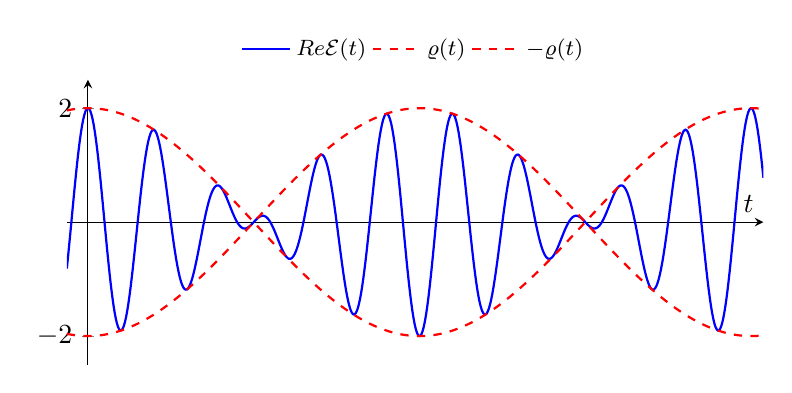
\begin{tikzpicture}
\begin{axis}[
  width=0.86\textwidth, height=5.2cm,
  axis lines=middle,
  xlabel={$t$},
  xmin=-0.4, xmax=12.8, ymin=-2.5, ymax=2.5,
  xtick=\empty, ytick={-2,0,2},
  samples=600, domain=-0.4:12.8,
  legend style={at={(0.5,1.03)},anchor=south,legend columns=3,draw=none,font=\footnotesize}
]
\addplot[blue,thick] {2*cos(deg(0.5*x))*cos(deg(5*x))};
\addplot[red,dashed,thick] {2*abs(cos(deg(0.5*x)))};
\addplot[red,dashed,thick] {-2*abs(cos(deg(0.5*x)))};
\legend{$\operatorname{Re}\mathcal E(t)$,$\varrho(t)$,$-\varrho(t)$}
\end{axis}
\end{tikzpicture}
\caption{The envelope of a two-component beat: a fast carrier modulated by the slow envelope $2A|\cos(\Delta\omega t/2)|$. Here $A=1$, $\Delta\omega=1$ and $\bar\omega=5$.}
\label{fig:dyn_envelope_beat}
\end{figure}

\begin{remark}[Reconciliation with the audio and mechanical chapters]\label{rem:dyn_envelope_beat_convention}
The chapters `Periodic Structure of Audio Systems' and `Periodic Structure of Mechanical Systems' record the `envelope period' as $4\pi/\Delta\omega$ (\cref{lem:beat_periodic}, \cref{prop:beat_phenomenon}). Under \cref{def:dyn_envelope} that is the period of the \emph{signed} slowly varying factor; the period of the \emph{modulus} envelope is $2\pi/\Delta\omega$, equal to the beat period $T_{\text{beat}}=1/\Delta f$. With the present definition the two statements should be reconciled as follows: the beat period equals the modulus-envelope period, whilst the signed factor repeats only every two beat periods.
\end{remark}

\subsection{Difference frequencies and the periodicity of the envelope}

\begin{theorem}[Difference-frequency expansion]\label{thm:dyn_envelope_difference}
Let $\mathcal E(t)=\sum_{k=1}^{K}A_ke^{i(\omega_kt+\phi_k)}$, where $K\ge2$, $A_k>0$ are constants and $\omega_1,\dots,\omega_K$ are pairwise distinct. Then
\[
\varrho^2(t)=\sum_{k=1}^{K}A_k^2+2\sum_{1\le j<k\le K}A_jA_k\cos\bigl((\omega_j-\omega_k)t+(\phi_j-\phi_k)\bigr).
\]
Let $D$ be the additive subgroup generated by the difference frequencies $\omega_j-\omega_k$ whose coefficients on the right-hand side do not vanish. Then:
\begin{enumerate}[label=(\roman*)]
    \item the spectrum of $\varrho^2$ contains difference frequencies only; equivalently, the spectrum of $\varrho^2$ is the autocorrelation of the carrier spectrum (the discrete Wiener--Khinchin relation);
    \item if $D$ is discrete with $D=\omega_D\mathbb Z$ ($\omega_D>0$), then the least positive period of $\varrho$ is $T_{\text{env}}=2\pi/\omega_D$; if $D$ is not discrete, $\varrho$ is not periodic;
    \item if every $\omega_k\in\omega_0\mathbb Z$, then $T_{\text{env}}$ divides the carrier period $T_c=2\pi/\omega_0$.
\end{enumerate}
\end{theorem}

\begin{proof}
Expanding $\varrho^2=\mathcal E\overline{\mathcal E}$ gives
\[
\mathcal E\overline{\mathcal E}=\sum_{j,k=1}^{K}A_jA_k e^{i((\omega_j-\omega_k)t+(\phi_j-\phi_k))}.
\]
Separating the $K$ terms with $j=k$ (each equal to $A_k^2$) from those with $j\ne k$, and pairing the latter as $(j,k)$ and $(k,j)$, the identity $e^{i\theta}+e^{-i\theta}=2\cos\theta$ yields the expansion.

(i) is read off from the expansion. (ii) The expansion is a finite trigonometric polynomial whose non-zero frequencies generate $D$; a trigonometric polynomial has period $T$ if and only if $\nu T\in2\pi\mathbb Z$ for every non-zero frequency $\nu$ (by the linear independence of the characters). Hence the period group of $\varrho^2$ is $(2\pi/\omega_D)\mathbb Z$. Since $\varrho=\sqrt{\varrho^2}\ge0$, $T$ is a period of $\varrho^2$ if and only if it is a period of $\varrho$; the two therefore have the same period group, and the least positive period is $2\pi/\omega_D$. (iii) If $\omega_k\in\omega_0\mathbb Z$, then $D\subseteq\omega_0\mathbb Z$, so $\omega_D$ is a positive integer multiple of $\omega_0$ and $T_{\text{env}}=2\pi/\omega_D$ divides $2\pi/\omega_0$.
\end{proof}

\begin{corollary}[A quasi-periodic carrier may have a periodic envelope]\label{cor:dyn_envelope_quasiperiodic}
Let $\mathcal E(t)=Ae^{i\omega_1t}+Ae^{i\omega_2t}$ with $A>0$ and $\omega_1/\omega_2\notin\mathbb Q$. Then $\mathcal E$ is not periodic (it is a Bohr quasi-periodic function), yet $\varrho$ has least positive period $2\pi/|\omega_1-\omega_2|$.
\end{corollary}

\begin{proof}
A sum of two exponentials with incommensurate frequencies has no non-zero period: if $T$ were a period of $\mathcal E$, the linear independence of the characters would give $e^{i\omega_1T}=e^{i\omega_2T}=1$, hence $\omega_1T,\omega_2T\in2\pi\mathbb Z$, contradicting $\omega_1/\omega_2\notin\mathbb Q$. The periodicity of the envelope is given by \cref{thm:dyn_envelope_difference}(ii), with $D=|\omega_1-\omega_2|\mathbb Z$.
\end{proof}

\begin{remark}[Envelope periodicity is strictly weaker than carrier periodicity]\label{rem:dyn_envelope_weaker}
\cref{cor:dyn_envelope_quasiperiodic} shows that $\mathcal E$ periodic $\Rightarrow$ $\varrho$ periodic (since $\varrho=|\mathcal E|$), but not conversely. The group-theoretic reason is clear: the envelope is invariant under the common phase rotation $U(1)$ (\cref{prop:dyn_envelope_sup}) and sees only the \emph{relative} phases $\Theta_j-\Theta_k$, the common fast phase having been quotiented out. The period of the envelope is thus the `closure period of the relative phases'; it may be coarser than the carrier period, and it may exist even when the carrier has no period at all.
\end{remark}

\subsection{The period-difference density}
\label{subsec:dyn_period_difference_density}

This subsection writes the `period difference of two periodic functions' as an integrable density. There are two requirements:
\begin{enumerate}[label=(\roman*)]
    \item \textbf{pointwise}: given \(f,g\) and a point \(x\), return the period-difference density at \(x\);
    \item \textbf{integral}: integrated over an interval \([a,b]\), return the period difference over that interval.
\end{enumerate}
These two requirements force the pointwise value to be a dimensionless density rather than a period, and make an interval normalisation unavoidable.

\begin{remark}[Why the pointwise value cannot be a period]
\label{rem:dyn_period_density_no_go}
If \(D(x)\) were a period (with the dimension of time), then \(\int_a^b D(x)\,dx\) would have the dimension of time\(^2\) and could not equal a period difference (time). More strictly, if \(D(x)\) were fixed and
\[
\int_a^b D(x)\,dx=T_f-T_g
\]
for every interval \([a,b]\), then the integral over every subinterval would be the same constant; differentiating with respect to \(b\) gives \(D(b)=0\) for almost every \(b\), a contradiction. Hence the pointwise value must be a dimensionless density, and interval normalisation is unavoidable; `the period difference over an interval' should be read as the difference of the interval-averaged periods, or as `one period difference accumulated per beat'.
\end{remark}

\textbf{The general interval version.}

Let \(f,g\) have global least positive periods \(T_f,T_g\), with \(T_f>T_g\) (otherwise interchange \(f,g\)). Let their analytic phases be \(\Theta_f,\Theta_g\) and their local frequencies
\[
f_f(x)=\frac{\dot\Theta_f(x)}{2\pi},\qquad
f_g(x)=\frac{\dot\Theta_g(x)}{2\pi}.
\]
On the interval \([a,b]\) define the cycle counts
\[
N_f=\int_a^b f_f(x)\,dx,\qquad
N_g=\int_a^b f_g(x)\,dx,
\]
and the interval-averaged periods
\[
T_f^{[a,b]}=\frac{b-a}{N_f},\qquad
T_g^{[a,b]}=\frac{b-a}{N_g}.
\]

\begin{definition}[Frequency-difference and interval period-difference densities]
\label{def:dyn_period_difference_density}
Call
\[
\Delta_{f,g}(x)=f_g(x)-f_f(x)
\]
the \textbf{frequency-difference density} of \(f,g\), and
\[
D_{f,g}(x;a,b)=\frac{b-a}{N_fN_g}\Delta_{f,g}(x)
\]
the \textbf{period-difference density} of \(f,g\) on the interval \([a,b]\).
\end{definition}

\begin{proposition}[Integral over an interval]
\label{prop:dyn_period_difference_integral}
For any interval \([a,b]\),
\[
\int_a^b D_{f,g}(x;a,b)\,dx
=(b-a)\left(\frac1{N_f}-\frac1{N_g}\right)
=T_f^{[a,b]}-T_g^{[a,b]}.
\]
\end{proposition}

\begin{proof}
By the definition of \(D_{f,g}\),
\[
\int_a^b D_{f,g}(x;a,b)\,dx
=\frac{b-a}{N_fN_g}\int_a^b\Delta_{f,g}(x)\,dx
=\frac{b-a}{N_fN_g}(N_g-N_f),
\]
which rearranges to \((b-a)(1/N_f-1/N_g)=T_f^{[a,b]}-T_g^{[a,b]}\).
\end{proof}

\textbf{The beat-period special case.}

Take the common interval to be one beat period
\[
T_{\rm env}=\frac{T_fT_g}{T_f-T_g}.
\]
Then \(N_f=T_{\rm env}/T_f\), \(N_g=T_{\rm env}/T_g\) and \(N_g-N_f=1\). The normalisation factor becomes
\[
\frac{T_{\rm env}}{N_fN_g}=T_f-T_g,
\]
the density becomes
\[
D_{f,g}(x)=(T_f-T_g)\bigl(f_g(x)-f_f(x)\bigr),
\]
and
\[
\int_0^{T_{\rm env}}D_{f,g}(x)\,dx
=(T_f-T_g)(N_g-N_f)=T_f-T_g.
\]
More generally, an interval containing \(m\) beat periods gives \(m(T_f-T_g)\); this is `one period difference accumulated per beat'.

\textbf{The role of the envelope.} In the narrowband/two-tone case the envelope \(|z_f+z_g|\) has period exactly \(T_{\rm env}\), marking the interval over which the phase difference completes \(2\pi\) (\cref{def:dyn_envelope}, \cref{prop:dyn_envelope_beat}). The envelope supplies the integration domain/clock; the local frequency (phase) supplies the pointwise density. The envelope alone does not give \(D_{f,g}(x)\), and the phase alone does not give the simple beat scale, but \(T_{\rm env}\) can be computed from \(T_f,T_g\).

\begin{example}[Pure-tone check]
\label{ex:dyn_period_difference_pure_tone}
For \(f=\cos(2\pi x/T_f)\) and \(g=\cos(2\pi x/T_g)\), \(f_f=1/T_f\) and \(f_g=1/T_g\), so
\[
D_{f,g}(x)=\frac{(T_f-T_g)^2}{T_fT_g}
\]
is constant; over \(T_{\rm env}=T_fT_g/(T_f-T_g)\),
\[
\frac{(T_f-T_g)^2}{T_fT_g}\cdot\frac{T_fT_g}{T_f-T_g}=T_f-T_g,
\]
in agreement with direct subtraction.
\end{example}

\begin{remark}[Calibration for arbitrary periodic functions]
\label{rem:dyn_period_density_calibration}
For signals with rich harmonics or zeros, the winding number of the analytic phase may not be \(1\). In that case replace \(\dot\Theta/(2\pi)\) by a \textbf{calibrated local frequency} \(f_f(x)\) satisfying
\[
\int_0^{T_f} f_f(x)\,dx=1.
\]
It may be obtained from an STFT ridge, an autocorrelation, or the instantaneous frequency divided by its integral/winding number over one period. After calibration, the integral identities above do not depend on the local details of the analytic phase, only on the total cycle counts.
\end{remark}

\begin{remark}[Division of labour between the two densities]
\label{rem:dyn_two_densities}
\(\Delta_{f,g}\) counts the `extra cycles' and is a dimensionless frequency difference; \(D_{f,g}\) multiplies it by the interval normalisation factor \((b-a)/(N_fN_g)\), so that its integral over \([a,b]\) becomes the interval period difference (on the beat period this factor becomes \(T_f-T_g\)). The envelope supplies the beat clock \(T_{\rm env}\); the phase difference supplies the density. The density \(D(t)=1/L_m-1/L_z\) in the calendar chapter is a calendar instance of \(\Delta_{f,g}\) (used to count intercalary excess); multiplying it by the corresponding interval normalisation factor gives \(D_{f,g}\), which explains the time difference. The period-difference density is therefore not a calendar-specific construction but a general object of the analytic signal.
\end{remark}

\subsection{Modulation order and commensurability}

\begin{definition}[Modulation order]\label{def:dyn_modulation_order}
For the two-component signal of \cref{prop:dyn_envelope_beat}(ii), the \textbf{modulation order} is
\[
N:=\frac{T_{\text{env}}}{T_c}=\frac{\bar\omega}{\Delta\omega},
\]
where $T_c=2\pi/\bar\omega$ is the carrier period.
\end{definition}

\begin{proposition}[Modulation order and commensurability]\label{prop:dyn_modulation_order}
For the two-component signal of \cref{prop:dyn_envelope_beat}(ii):
\begin{enumerate}[label=(\roman*)]
    \item $\mathcal E$ is periodic if and only if $N\in\mathbb Q$;
    \item if $N=p/q$ with $p,q$ coprime, then the least positive period of $\mathcal E$ is $mT_{\text{env}}$, where $m$ is a positive integer with $m\mid 2q$.
\end{enumerate}
\end{proposition}

\begin{proof}
(i) $\mathcal E$ is a sum of two exponentials whose frequency ratio is
\[
\frac{\omega_2}{\omega_1}=\frac{2N+1}{2N-1}.
\]
Such a sum has period $T>0$ if and only if $\omega_1T,\omega_2T\in2\pi\mathbb Z$, which requires $\omega_1/\omega_2\in\mathbb Q$; conversely, if $\omega_1/\omega_2=r\in\mathbb Q$, then $T=2\pi/\gcd(\omega_1,\omega_2)$ is a period. And $(2N+1)/(2N-1)\in\mathbb Q$ if and only if $N\in\mathbb Q$.

(ii) Take $T_0=qT_{\text{env}}=2\pi q/\Delta\omega$. Then $\bar\omega T_0=2\pi qN=2\pi p$ and $\Delta\omega T_0/2=\pi q$, so by \cref{prop:dyn_envelope_beat}(ii),
\[
\mathcal E(t+T_0)=(-1)^q\mathcal E(t).
\]
Hence $2T_0=2qT_{\text{env}}$ is a period of $\mathcal E$. Let $P$ be the least positive period of $\mathcal E$. Since $P$ is also a period of $\varrho$, whose least positive period is $T_{\text{env}}$, we have $P=mT_{\text{env}}$ with $m\in\mathbb N^+$. Since $P\mid 2qT_{\text{env}}$, it follows that $m\mid 2q$.
\end{proof}

\begin{remark}[Interface with intercalation and continued fractions]\label{rem:dyn_envelope_intercalation}
\cref{prop:dyn_modulation_order} reduces the question `is the two-component signal periodic?' to `is the modulation order $N$ rational?'. The irrationality of $N$ is measured by its continued-fraction convergents $p_j/q_j$: for $N\approx p_j/q_j$ the signal closes approximately after $q_j$ envelope periods, with residual phase error $2\pi q_j|N-p_j/q_j|$, which by the theory of continued fractions does not exceed $2\pi/q_{j+1}$. This is the same type of problem as the approximation of the period ratio $\varrho$ by continued fractions in the chapter `Discrete Sampling, Congruence Angles and Intercalation' (\cref{thm:continued_fraction_best_approx_parallel})---there the ratio of sampling window to signal is approximated, here the ratio of carrier to envelope.
\end{remark}

\subsection{Interfaces and open problems}

\begin{remark}[Interfaces with other chapters]\label{rem:dyn_envelope_interfaces}
The envelope recurs under different names in later chapters:
\begin{enumerate}[label=(\roman*)]
    \item \textbf{beats} (\cref{lem:beat_periodic}, \cref{prop:beat_phenomenon}): the modulus envelope of two close frequencies;
    \item \textbf{leakage envelope} (\cref{thm:leakage_envelope_parallel}): the decay profile of the sidelobes of a window kernel, an envelope in the frequency domain;
    \item \textbf{analytic signal} (\cref{prop:analytic_signal}): the Hilbert envelope of a real signal;
    \item \textbf{wave packet} (\cref{ex:dispersive_pulse}): the envelope of a Gaussian pulse travels at the group velocity, and dispersion acts on the envelope rather than on the carrier;
    \item \textbf{slow--fast systems} (\cref{prop:pdo_enso_separation}): the modulation of the amplitude of a fast oscillation by a slow variable, i.e.\ envelope dynamics;
    \item \textbf{business cycles}: the modulation of Kitchin-cycle amplitude by the Juglar cycle (chapter `Periodic Structure of Economic Systems').
\end{enumerate}
\end{remark}

\begin{remark}[Open problems]\label{rem:dyn_envelope_open}
\begin{enumerate}[label=(\alph*)]
    \item \textbf{Uniqueness of the multi-component envelope}: when $\mathcal E$ contains several incommensurate difference frequencies, $\varrho$ is quasi-periodic; how should its `envelope of the envelope' be defined, and is there a unique two-scale decomposition?
    \item \textbf{Error bounds for envelope extraction}: how can the discrepancy between the Hilbert envelope, the peak envelope and the modulus envelope of \cref{def:dyn_envelope} be quantified under finite sampling?
    \item \textbf{Categorical description}: can the envelope, as a functor of $U(1)$-invariants, be incorporated into the framework of the chapter `Periodic Category'?
\end{enumerate}
\end{remark}

\section{Three dynamic epicycle groups}
\label{sec:dyn_triple}

\subsection{Basic definitions}

\begin{definition}[Three dynamic epicycle groups]\label{def:dyn_triple_groups}
Let there be three mutually independent dynamic epicycle groups
\[
T(t)=\sum_{k=1}^{K_T}A_k(t)e^{i(\omega_k(t)t+\phi_k(t))},
\]
\[
S(t)=\sum_{l=1}^{K_S}B_l(t)e^{i(\nu_l(t)t+\psi_l(t))},
\]
\[
O(t)=\sum_{m=1}^{K_O}C_m(t)e^{i(\mu_m(t)t+\chi_m(t))},
\]
called the \textbf{time group}, the \textbf{space group} and the \textbf{observer group} respectively. The parameters of all three groups are $C^1$ functions.
\end{definition}

\begin{definition}[Synthesis--projection observation result]\label{def:dyn_triple_projection}
Define the \textbf{composite trajectory} to be $T(t)+S(t)$, and define the \textbf{observation result} to be the real part of the bilinear pairing of the composite trajectory with the observer group:
\[
\boxed{\ \mathcal O(t)=\operatorname{Re}\!\big[(T(t)+S(t))\,\overline{O(t)}\big]\ }.
\]
\end{definition}

\begin{remark}[Relation to the static model of the `Vector analysis' chapter]\label{rem:dyn_triple_static_relation}
\cref{def:dyn_triple_projection} is the dynamic generalisation of the threefold static projection model of the `Vector Analysis' chapter: when the parameters of all three groups are constant, the two coincide completely.
\end{remark}

\subsection{Basic properties}

\begin{proposition}[Additivity of synthesis--projection]\label{prop:dyn_triple_additivity}
The observation result is additive with respect to the time group and the space group:
\[
\mathcal O(t)=\operatorname{Re}[T(t)\overline{O(t)}]+\operatorname{Re}[S(t)\overline{O(t)}].
\]
\end{proposition}

\begin{proof}
By the distributivity of complex multiplication $(T+S)\overline O=T\overline O+S\overline O$, and then by the linearity of the real part.
\end{proof}

\begin{proposition}[Degeneracy for a unit-modulus observer]\label{prop:dyn_triple_unimodular}
If $O(t)=e^{i\chi(t)}$, then \cref{def:dyn_triple_projection} degenerates to
\[
\mathcal O(t)=\operatorname{Re}\!\big[(T(t)+S(t))\,e^{-i\chi(t)}\big],
\]
in agreement with the form of the single-group dynamic projection \cref{def:dyn_projection}.
\end{proposition}

\begin{proof}
When $|O(t)|=1$ we have $\overline{O(t)}=O(t)^{-1}=e^{-i\chi(t)}$; substituting gives the result.
\end{proof}

\begin{lemma}[Bilinear pairing and modulus weighting]\label{lem:dyn_triple_weight}
In the general case,
\[
\mathcal O(t)=\operatorname{Re}\!\big[(T(t)+S(t))\,\overline{\widehat O(t)}\big]\cdot|O(t)|,
\qquad \widehat O(t)=O(t)/|O(t)|.
\]
\end{lemma}

\begin{proof}
Let $\widehat O=O/|O|$; then $O=|O|\widehat O$ and $\overline O=|O|\overline{\widehat O}$. Substituting,
\[
(T+S)\overline O=|O|\cdot(T+S)\overline{\widehat O}.
\]
Taking the real part and pulling out the real factor $|O|\ge 0$ gives the result.
\end{proof}

\begin{theorem}[Continuity of the three-group dynamic projection]\label{thm:dyn_triple_continuity}
Let the parameters of $T,S,O$ all be $C^1$ functions. Then $\mathcal O(t)$ is a $C^1$ function. If $O(t)\neq 0$ for all $t$, then $\mathcal O(t)$ and $|O(t)|$ have the same zero set.
\end{theorem}

\begin{proof}
\textbf{Continuity}: $\mathcal O$ is the real part of a product of the $C^1$ functions $T,S,O$ and their conjugates, hence is $C^1$.

\textbf{Zero set}: By \cref{lem:dyn_triple_weight}, $\mathcal O=|O|\cdot\operatorname{Re}[(T+S)\overline{\widehat O}]$. If $|O(t)|\neq 0$, then $\mathcal O(t)=0$ if and only if $\operatorname{Re}[(T+S)\overline{\widehat O}]=0$.
\end{proof}

\begin{corollary}[Beat-frequency formula for three single frequencies]\label{cor:dyn_triple_beat}
Take $T(t)=A e^{i\omega t}$, $S(t)=B e^{i\nu t}$, $O(t)=C e^{i\mu t}$ ($A,B,C>0$). Then
\[
\mathcal O(t)=AC\cos((\omega-\mu)t)+BC\cos((\nu-\mu)t).
\]
When $|\omega-\nu|$ is very small a beat arises, with beat period $T_{\text{beat}}=2\pi/|\omega-\nu|$.
\end{corollary}

\begin{proof}
$T\overline O=AC e^{i(\omega-\mu)t}$, $S\overline O=BC e^{i(\nu-\mu)t}$; adding and taking the real part gives the result.
\end{proof}

\begin{property}[Basic properties of the three-group dynamic projection]\label{prop:dyn_triple_properties}
\begin{enumerate}[label=(\roman*)]
    \item \textbf{Linearity}: for fixed $O$, $\mathcal O$ is real-linear in $T$ and $S$.
    \item \textbf{Observer sign reversal}: $O\mapsto-O$ sends $\mathcal O\mapsto-\mathcal O$.
    \item \textbf{Observer conjugation}: $O\mapsto\overline O$ sends $\mathcal O\mapsto\operatorname{Re}[(T+S)O]$.
    \item \textbf{Energy decomposition}: $|\mathcal O(t)|\le|T(t)+S(t)|\cdot|O(t)|$.
\end{enumerate}
\end{property}

\begin{proof}
(i) By \cref{prop:dyn_triple_additivity} and the linearity of complex multiplication in its first factor. (ii) $\overline{-O}=-\overline O$. (iii) $\overline{\overline O}=O$. (iv) $|\mathcal O|\le|(T+S)\overline O|=|T+S|\cdot|O|$.
\end{proof}

\begin{example}[Beat-frequency example of the three-group dynamic projection]\label{ex:dyn_triple_beat_example}
Take $T(t)=e^{i10t}$, $S(t)=e^{i12t}$, $O(t)=e^{i11t}$. By \cref{cor:dyn_triple_beat},
\[
\mathcal O(t)=\cos(-t)+\cos(t)=2\cos t.
\]
The beat period is $T_{\text{beat}}=2\pi$.
\end{example}

\begin{remark}[Normalised and unnormalised observers]\label{rem:dyn_triple_normalisation}
If the observer group is normalised to $\widehat O=O/|O|$, then the weight factor $|O(t)|$ in \cref{lem:dyn_triple_weight} disappears, and the observation result degenerates to a genuine orthogonal projection. Whether or not to normalise is a modelling choice.
\end{remark}

\section{Rotating three planes}
\label{sec:dyn_rotating_planes}

\subsection{Basic definitions}

\begin{definition}[Rotating three planes]\label{def:dyn_rotating_planes}
Let there be three mutually independent complex planes $\mathbb C_T,\mathbb C_S,\mathbb C_O$. On each plane there is a dynamic epicycle group $T_0(t),S_0(t),O_0(t)$ (as in \cref{def:dyn_triple_groups}). Let $\theta_T,\theta_S,\theta_O:\mathbb R\to\mathbb R$ be $C^1$ functions. Define the \textbf{rotated trajectories} by
\[
T(t)=T_0(t)e^{i\theta_T(t)},\quad
S(t)=S_0(t)e^{i\theta_S(t)},\quad
O(t)=O_0(t)e^{i\theta_O(t)}.
\]
The rotation angles of the three planes are determined by the epicycle group in the corresponding plane, hence the phrase `rotation according to the properties of the internal epicycle'.
\end{definition}

\begin{figure}[htbp]
\centering
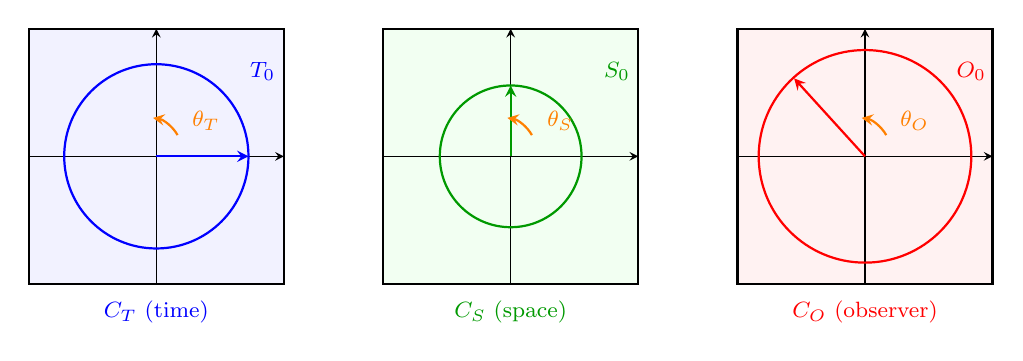
\begin{tikzpicture}[scale=0.9,>=stealth]
  % Three complex planes
  \begin{scope}[shift={(0,0)}]
    \draw[thick, fill=blue!5] (-1.8,-1.8) rectangle (1.8,1.8);
    \draw[->] (-1.8,0) -- (1.8,0);
    \draw[->] (0,-1.8) -- (0,1.8);
    \draw[thick,blue] (0,0) circle (1.3);
    \draw[->,thick,blue] (0,0) -- (1.3,0);
    \node[blue,font=\footnotesize] at (0,-2.2) {$\mathbb C_T$ (time)};
    \node[blue,font=\footnotesize] at (1.5,1.2) {$T_0$};
  \end{scope}
  \begin{scope}[shift={(5,0)}]
    \draw[thick, fill=green!5] (-1.8,-1.8) rectangle (1.8,1.8);
    \draw[->] (-1.8,0) -- (1.8,0);
    \draw[->] (0,-1.8) -- (0,1.8);
    \draw[thick,green!60!black] (0,0) circle (1.0);
    \draw[->,thick,green!60!black] (0,0) -- (0,1.0);
    \node[green!60!black,font=\footnotesize] at (0,-2.2) {$\mathbb C_S$ (space)};
    \node[green!60!black,font=\footnotesize] at (1.5,1.2) {$S_0$};
  \end{scope}
  \begin{scope}[shift={(10,0)}]
    \draw[thick, fill=red!5] (-1.8,-1.8) rectangle (1.8,1.8);
    \draw[->] (-1.8,0) -- (1.8,0);
    \draw[->] (0,-1.8) -- (0,1.8);
    \draw[thick,red] (0,0) circle (1.5);
    \draw[->,thick,red] (0,0) -- (-1.0,1.1);
    \node[red,font=\footnotesize] at (0,-2.2) {$\mathbb C_O$ (observer)};
    \node[red,font=\footnotesize] at (1.5,1.2) {$O_0$};
  \end{scope}
  % Rotation labels
  \draw[->,thick,orange] (0.3,0.3) arc (30:80:0.5);
  \node[orange,font=\footnotesize] at (0.7,0.5) {$\theta_T$};
  \draw[->,thick,orange] (5.3,0.3) arc (30:80:0.5);
  \node[orange,font=\footnotesize] at (5.7,0.5) {$\theta_S$};
  \draw[->,thick,orange] (10.3,0.3) arc (30:80:0.5);
  \node[orange,font=\footnotesize] at (10.7,0.5) {$\theta_O$};
\end{tikzpicture}
\caption{Rotating three planes: the three independent complex planes each rotate according to the properties of the internal epicycle, with rotation angles $\theta_T,\theta_S,\theta_O$.}
\label{fig:dyn_rotating_planes}
\end{figure}

\begin{definition}[Observation result for the rotating three planes]\label{def:dyn_rotating_planes_projection}
Continuing with \cref{def:dyn_rotating_planes}, define
\[
\boxed{\ \mathcal O(t)=\operatorname{Re}\!\big[(T(t)+S(t))\,\overline{O(t)}\big]\ }.
\]
Expanding:
\[
\mathcal O(t)=\operatorname{Re}\!\big[(T_0 e^{i\theta_T}+S_0 e^{i\theta_S})\,e^{-i\theta_O}\,\overline{O_0}\big].
\]
\end{definition}

\subsection{Basic properties}

\begin{proposition}[Phase-shift action of the rotation angles]\label{prop:dyn_rotation_phase_shift}
The rotating three planes are equivalent to applying the phase shifts $\theta_T,\theta_S,\theta_O$ to $T_0,S_0,O_0$ respectively before composition:
\[
\mathcal O(t)=\operatorname{Re}\!\big[(T_0 e^{i(\theta_T-\theta_O)}+S_0 e^{i(\theta_S-\theta_O)})\,\overline{O_0}\big].
\]
Hence only the two relative rotation angles $\theta_T-\theta_O$ and $\theta_S-\theta_O$ take effect.
\end{proposition}

\begin{proof}
Expanding,
\[
(T_0 e^{i\theta_T}+S_0 e^{i\theta_S})\overline{O_0 e^{i\theta_O}}
=(T_0 e^{i\theta_T}+S_0 e^{i\theta_S})\overline{O_0}e^{-i\theta_O}.
\]
Distributing $e^{-i\theta_O}$ over each term gives
\[
=T_0 e^{i(\theta_T-\theta_O)}\overline{O_0}+S_0 e^{i(\theta_S-\theta_O)}\overline{O_0}
=\big[T_0 e^{i(\theta_T-\theta_O)}+S_0 e^{i(\theta_S-\theta_O)}\big]\overline{O_0}.
\]
Taking the real part gives the result.
\end{proof}

\begin{theorem}[Invariant under synchronous rotation]\label{thm:dyn_sync_invariance}
If $\theta_T(t)=\theta_S(t)=\theta_O(t)=\theta(t)$, then the observation result is the same as in the static case:
\[
\mathcal O(t)=\operatorname{Re}\!\big[(T_0(t)+S_0(t))\overline{O_0(t)}\big].
\]
\end{theorem}

\begin{proof}
Substituting $\theta_T=\theta_S=\theta_O=\theta$, by \cref{prop:dyn_rotation_phase_shift} both relative angles are zero:
\[
T_0 e^{i0}+S_0 e^{i0}=T_0+S_0.
\]
Hence $\mathcal O=\operatorname{Re}[(T_0+S_0)\overline{O_0}]$, independently of $\theta$.
\end{proof}

\begin{corollary}[Frequency shift under asynchronous rotation]\label{cor:dyn_async_beat}
Take all three planes to be single-frequency: $T_0=A e^{i\omega t}$, $S_0=B e^{i\nu t}$, $O_0=C e^{i\mu t}$, with rotation angles $\theta_j(t)=\Omega_j t$. Then
\[
\mathcal O(t)=AC\cos\big((\omega+\Omega_T-\mu-\Omega_O)t\big)+BC\cos\big((\nu+\Omega_S-\mu-\Omega_O)t\big).
\]
\end{corollary}

\begin{proof}
By \cref{prop:dyn_rotation_phase_shift}, $T_0e^{i(\theta_T-\theta_O)}=A e^{i(\omega+\Omega_T-\Omega_O)t}$ and $S_0e^{i(\theta_S-\theta_O)}=B e^{i(\nu+\Omega_S-\Omega_O)t}$. Substituting and taking the real part gives the result.
\end{proof}

\begin{property}[Basic properties of the rotating three planes]\label{prop:dyn_rotating_planes_properties}
\begin{enumerate}[label=(\roman*)]
    \item \textbf{Relativity}: the observation result depends only on the relative rotation angles $\theta_T-\theta_O$ and $\theta_S-\theta_O$.
    \item \textbf{Synchronous invariance}: when the three planes rotate synchronously, the observation result is unchanged.
    \item \textbf{Frequency translation}: if $\theta_j=\Omega_j t$, then all component frequencies in plane $j$ are translated by $\Omega_j$ as a whole.
\end{enumerate}
\end{property}

\begin{proof}
(i)(ii) By \cref{prop:dyn_rotation_phase_shift} and \cref{thm:dyn_sync_invariance}. (iii) Directly from $e^{i(\omega_j t+\Omega_j t)}=e^{i(\omega_j+\Omega_j)t}$.
\end{proof}

\begin{example}[Beat-frequency example of asynchronously rotating three planes]\label{ex:dyn_rotating_planes_example}
Take $T_0=e^{i10t}$, $S_0=e^{i12t}$, $O_0=e^{i11t}$, $\theta_T=0.5t$, $\theta_S=0$, $\theta_O=0$. By \cref{cor:dyn_async_beat},
\[
\mathcal O(t)=\cos(-0.5t)+\cos(t).
\]
The two terms have frequencies $0.5$ and $1$ respectively, producing a slow beat.
\end{example}

\begin{remark}[Choice of rotation angle]\label{rem:dyn_rotation_angle_choice}
`Rotation according to the properties of the internal epicycle' admits several implementations: $\theta_j(t)=\omega_{j,1}(t)t$, $\theta_j(t)=\arg X_j(t)$, $\theta_j(t)=\sum_k\omega_{j,k}(t)t$, and so on. This chapter does not fix one of them; all the conclusions hold for an arbitrary $C^1$ rotation angle.
\end{remark}

\section{Quaternion episphere groups}
\label{sec:dyn_quaternion_single}

\subsection{Basic definitions}

\begin{definition}[Quaternion episphere group]\label{def:dyn_quaternion_group}
Let $K_T,K_S,K_O\in\mathbb N^+$. Let $a_k,b_l,c_m:\mathbb R\to\mathbb R$ be $C^1$ real-valued functions; let $\mathbf u_k,\mathbf v_l,\mathbf w_m:\mathbb R\to S^2$ be $C^1$ functions taking values in the unit pure imaginary quaternions; and let $\theta_k,\psi_l,\chi_m:\mathbb R\to\mathbb R$ be $C^1$ functions. Define
\[
q_T(t)=\sum_{k=1}^{K_T}a_k(t)e^{\mathbf u_k(t)\theta_k(t)},\quad
q_S(t)=\sum_{l=1}^{K_S}b_l(t)e^{\mathbf v_l(t)\psi_l(t)},\quad
q_O(t)=\sum_{m=1}^{K_O}c_m(t)e^{\mathbf w_m(t)\chi_m(t)}.
\]
They are called the \textbf{time episphere group}, the \textbf{space episphere group} and the \textbf{observer episphere group} respectively.
\end{definition}

\begin{definition}[Synthesis--projection observation result]\label{def:dyn_quaternion_projection}
Define the composite vector to be $q_T(t)+q_S(t)$; the observation result is
\[
\boxed{\ \mathcal Q(t)=\operatorname{Re}\!\big[(q_T(t)+q_S(t))\,\overline{q_O(t)}\big]\ }.
\]
Here $\overline{q_O}$ is the quaternion conjugate and $\operatorname{Re}$ takes the scalar part of the quaternion.
\end{definition}

\begin{remark}[Relation to the static model of the `Vector analysis' chapter]\label{rem:dyn_quaternion_static_relation}
\cref{def:dyn_quaternion_projection} is the dynamic version of the static projection model of the `Vector Analysis' chapter under the `compose first, then project' convention.
\end{remark}

\subsection{Basic properties}

\begin{proposition}[Distinction between scalar projection and conjugation projection]\label{prop:dyn_quaternion_projection_types}
The scalar part of the quaternion inner product $\operatorname{Re}[q\overline{p}]$ and the conjugation action $p^{-1}qp$ are two different kinds of `projection':
\begin{enumerate}[label=(\roman*)]
    \item $\operatorname{Re}[q\overline{p}]$ is the inner-product projection on $\mathbb R^4$, and outputs a real number.
    \item $p^{-1}qp$ is a rotation of $SO(3)$, and outputs a quaternion.
\end{enumerate}
This chapter adopts (i).
\end{proposition}

\begin{proof}
(i) By the definition of the quaternion inner product, $\operatorname{Re}[q\overline p]=\sum_{i=0}^3 q_i p_i\in\mathbb R$.

(ii) Take $q=\mathbf i$ and $p=\mathbf j$. Then $p^{-1}=\overline p/|p|^2=-\mathbf j$, so
\[
p^{-1}qp=(-\mathbf j)\mathbf i\mathbf j.
\]
From $\mathbf i\mathbf j=\mathbf k$ and $\mathbf j\mathbf i=-\mathbf k$:
\[
(-\mathbf j)\mathbf i\mathbf j=(-\mathbf j)(\mathbf i\mathbf j)=(-\mathbf j)\mathbf k=-\mathbf j\mathbf k=-\mathbf i.
\]
Hence $p^{-1}qp=-\mathbf i\neq\mathbf i=q$; the conjugation action changes the quaternion.
\end{proof}

\begin{lemma}[Symmetry of the quaternion inner product]\label{lem:dyn_quaternion_inner_symmetry}
For any $p,q\in\mathbb H$, $\operatorname{Re}[p\overline q]=\operatorname{Re}[q\overline p]$.
\end{lemma}

\begin{proof}
The scalar part of $p\overline q$ is $p_0q_0+p_1q_1+p_2q_2+p_3q_3$ (the vector parts and the non-commutative terms do not affect the scalar part). This is a symmetric real bilinear form, hence $\operatorname{Re}[p\overline q]=\operatorname{Re}[q\overline p]$.
\end{proof}

\begin{theorem}[Non-commutative synthesis and observation order]\label{thm:dyn_quaternion_noncommutative}
Consider the additive synthesis $X_+=q_T+q_S$ and the multiplicative synthesis $X_\times=q_Tq_S$. Then in general $\operatorname{Re}[X_+\overline{q_O}]\neq\operatorname{Re}[X_\times\overline{q_O}]$, and $q_Tq_S\neq q_Sq_T$.
\end{theorem}

\begin{proof}
Take $q_T=\mathbf i$, $q_S=\mathbf j$ and $q_O=\mathbf k$.

Addition: $X_+=\mathbf i+\mathbf j$, so
\[
X_+\overline{q_O}=(\mathbf i+\mathbf j)(-\mathbf k)=-\mathbf i\mathbf k-\mathbf j\mathbf k.
\]
From $\mathbf i\mathbf k=-\mathbf j$ and $\mathbf j\mathbf k=\mathbf i$ we get $X_+\overline{q_O}=\mathbf j-\mathbf i$, whose scalar part is $0$.

Multiplication: $X_\times=\mathbf i\mathbf j=\mathbf k$, so
\[
X_\times\overline{q_O}=\mathbf k\cdot(-\mathbf k)=-\mathbf k^2=1,
\]
whose scalar part is $1$. Hence the two differ.

Non-commutativity: $\mathbf i\mathbf j=\mathbf k$ and $\mathbf j\mathbf i=-\mathbf k$, hence $\mathbf i\mathbf j\neq\mathbf j\mathbf i$.
\end{proof}

\begin{corollary}[Commutativity under the additive convention]\label{cor:dyn_quaternion_additive_commutative}
Under the additive convention, $\operatorname{Re}[(q_T+q_S)\overline{q_O}]=\operatorname{Re}[(q_S+q_T)\overline{q_O}]$.
\end{corollary}

\begin{proof}
Quaternion addition is commutative.
\end{proof}

\begin{property}[Basic properties of quaternion dynamic projection]\label{prop:dyn_quaternion_properties}
\begin{enumerate}[label=(\roman*)]
    \item \textbf{Real linearity}: for fixed $q_O$, $\mathcal Q$ is real-linear in $q_T$ and $q_S$.
    \item \textbf{Observer sign reversal}: $q_O\mapsto-q_O$ sends $\mathcal Q\mapsto-\mathcal Q$.
    \item \textbf{Norm bound}: $|\mathcal Q(t)|\le|q_T(t)+q_S(t)|\cdot|q_O(t)|$.
    \item \textbf{Scalar degeneracy}: if the quaternions degenerate to complex numbers, \cref{def:dyn_quaternion_projection} degenerates to \cref{def:dyn_triple_projection}.
\end{enumerate}
\end{property}

\begin{proof}
(i) By the linearity of quaternion addition, the anti-automorphism property of conjugation $(p+q)^* = p^*+q^*$ and the linearity of the scalar part.

(ii) $\overline{-q_O}=-\overline{q_O}$, and taking the scalar part changes the sign.

(iii) $|\mathcal Q|=|\operatorname{Re}[(q_T+q_S)\overline{q_O}]|\le|(q_T+q_S)\overline{q_O}|=|q_T+q_S|\cdot|q_O|$.

(iv) A complex number $z=x+iy$ embeds into the quaternions as $x+y\mathbf i$, and the scalar part of $z_1\overline{z_2}$ then agrees with the real part of the inner product in the complex case.
\end{proof}

\begin{example}[Single-sphere-group dynamic projection example]\label{ex:dyn_quaternion_example}
Take $q_T=e^{\mathbf i t}$, $q_S=e^{\mathbf j t}$ and $q_O=1$. Then
\[
\mathcal Q(t)=\operatorname{Re}[e^{\mathbf i t}+e^{\mathbf j t}]=\cos t+\cos t=2\cos t.
\]
\end{example}

\begin{remark}[Correspondence with the complex case]\label{rem:dyn_quaternion_complex_correspondence}
If all the quaternions are restricted to the same complex plane, the non-commutativity disappears, and \cref{def:dyn_quaternion_projection} degenerates completely to \cref{def:dyn_triple_projection}.
\end{remark}

\section{Rotating three-sphere groups}
\label{sec:dyn_quaternion_triple}

\subsection{Basic definitions}

\begin{definition}[Rotating three-sphere group]\label{def:dyn_rotating_quaternion_groups}
Let there be three mutually independent quaternion sphere groups $q_{T,0}(t),q_{S,0}(t),q_{O,0}(t)$. Let $r_T,r_S,r_O:\mathbb R\to S^3$ be $C^1$ functions taking values in the unit quaternions. Define
\[
q_T(t)=r_T(t)\,q_{T,0}(t)\,r_T(t)^{-1},\quad
q_S(t)=r_S(t)\,q_{S,0}(t)\,r_S(t)^{-1},\quad
q_O(t)=r_O(t)\,q_{O,0}(t)\,r_O(t)^{-1}.
\]
\end{definition}

\begin{figure}[htbp]
\centering
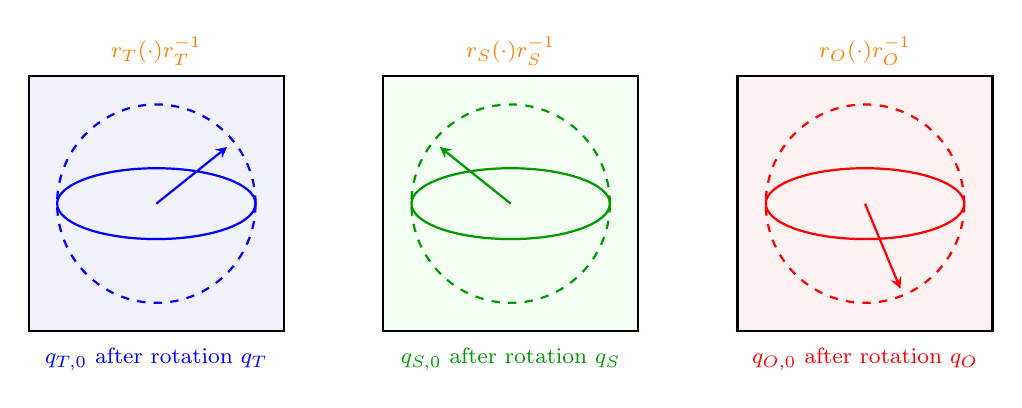
\begin{tikzpicture}[scale=0.9,>=stealth]

  \begin{scope}[shift={(0,0)}]
    \draw[thick, fill=blue!5] (-1.8,-1.8) rectangle (1.8,1.8);
    \draw[thick,blue,dashed] (0,0) circle (1.4);
    \draw[thick,blue] (0,0) ellipse (1.4 and 0.5);
    \draw[->,thick,blue] (0,0) -- (1.0,0.8);
    \node[blue,font=\footnotesize] at (0,-2.2) {$q_{T,0}$ after rotation $q_T$};
    \node[orange,font=\footnotesize] at (0,2.15) {$r_T(\cdot)r_T^{-1}$};
  \end{scope}

  \begin{scope}[shift={(5,0)}]
    \draw[thick, fill=green!5] (-1.8,-1.8) rectangle (1.8,1.8);
    \draw[thick,green!60!black,dashed] (0,0) circle (1.4);
    \draw[thick,green!60!black] (0,0) ellipse (1.4 and 0.5);
    \draw[->,thick,green!60!black] (0,0) -- (-1.0,0.8);
    \node[green!60!black,font=\footnotesize] at (0,-2.2) {$q_{S,0}$ after rotation $q_S$};
    \node[orange,font=\footnotesize] at (0,2.15) {$r_S(\cdot)r_S^{-1}$};
  \end{scope}

  \begin{scope}[shift={(10,0)}]
    \draw[thick, fill=red!5] (-1.8,-1.8) rectangle (1.8,1.8);
    \draw[thick,red,dashed] (0,0) circle (1.4);
    \draw[thick,red] (0,0) ellipse (1.4 and 0.5);
    \draw[->,thick,red] (0,0) -- (0.5,-1.2);
    \node[red,font=\footnotesize] at (0,-2.2) {$q_{O,0}$ after rotation $q_O$};
    \node[orange,font=\footnotesize] at (0,2.15) {$r_O(\cdot)r_O^{-1}$};
  \end{scope}

\end{tikzpicture}
\caption{Rotating three-sphere groups: the three quaternion sphere groups are rotated by the conjugation action of the unit quaternions $r_T,r_S,r_O$ respectively.}
\label{fig:dyn_rotating_quaternion_groups}
\end{figure}

\begin{definition}[Observation result for the rotating three-sphere groups]\label{def:dyn_rotating_quaternion_projection}
\[
\boxed{\ \mathcal Q(t)=\operatorname{Re}\!\big[(q_T(t)+q_S(t))\,\overline{q_O(t)}\big]\ }.
\]
\end{definition}

\subsection{Basic properties}

\begin{proposition}[Norm preservation under rotation]\label{prop:dyn_quaternion_rotation_norm}
For any unit quaternion $r$ and any $q\in\mathbb H$, $|rqr^{-1}|=|q|$.
\end{proposition}

\begin{proof}
By the multiplicativity of the quaternion norm $|pq|=|p|\cdot|q|$:
\[
|rqr^{-1}|=|r|\cdot|q|\cdot|r^{-1}|=|q|,
\]
where $|r|=1$ and $|r^{-1}|=|r|^{-1}=1$.
\end{proof}

\begin{lemma}[Conjugation preserves the scalar part]\label{lem:dyn_quaternion_conjugation_scalar}
For any unit quaternion $r$ and any $x\in\mathbb H$, $\operatorname{Re}[rxr^{-1}]=\operatorname{Re}[x]$.
\end{lemma}

\begin{proof}
Decompose $x$ as $x=x_0+\mathbf v$, with $x_0\in\mathbb R$ and $\mathbf v$ a pure imaginary quaternion. Then
\[
rxr^{-1}=r(x_0+\mathbf v)r^{-1}=x_0\cdot rr^{-1}+r\mathbf v r^{-1}=x_0+r\mathbf v r^{-1}.
\]
The scalar part is $x_0+\operatorname{Re}[r\mathbf v r^{-1}]$. Since the conjugation action preserves pure-imaginarity, $\operatorname{Re}[r\mathbf v r^{-1}]=0$. Hence $\operatorname{Re}[rxr^{-1}]=x_0=\operatorname{Re}[x]$.
\end{proof}

\begin{theorem}[Invariant under synchronous rotation]\label{thm:dyn_quaternion_sync_invariance}
If $r_T=r_S=r_O=r$, then
\[
\mathcal Q(t)=\operatorname{Re}\!\big[(q_{T,0}(t)+q_{S,0}(t))\overline{q_{O,0}(t)}\big].
\]
\end{theorem}

\begin{proof}
By \cref{def:dyn_rotating_quaternion_groups}, $q_T=rq_{T,0}r^{-1}$ and so on. Hence
\[
q_T+q_S=r(q_{T,0}+q_{S,0})r^{-1}.
\]
Conjugation: since $r$ is a unit quaternion, $r^{-1}=\overline r$, so
\[
\overline{q_O}=\overline{rq_{O,0}r^{-1}}=\overline{r^{-1}}\,\overline{q_{O,0}}\,\overline r=r\overline{q_{O,0}}r^{-1}.
\]
Substituting:
\[
\mathcal Q=\operatorname{Re}\big[r(q_{T,0}+q_{S,0})r^{-1}\cdot r\overline{q_{O,0}}r^{-1}\big]
=\operatorname{Re}\big[r(q_{T,0}+q_{S,0})\overline{q_{O,0}}r^{-1}\big].
\]
By \cref{lem:dyn_quaternion_conjugation_scalar}, taking $x=(q_{T,0}+q_{S,0})\overline{q_{O,0}}$, we get
\[
\mathcal Q=\operatorname{Re}\big[(q_{T,0}+q_{S,0})\overline{q_{O,0}}\big],
\]
independently of $r$.
\end{proof}

\begin{corollary}[Non-triviality under asynchronous rotation]\label{cor:dyn_quaternion_async}
If $r_T,r_S,r_O$ are not equal, then
\[
\mathcal Q(t)=\operatorname{Re}\!\big[r_T q_{T,0}r_T^{-1}\overline{r_O q_{O,0}r_O^{-1}}+r_S q_{S,0}r_S^{-1}\overline{r_O q_{O,0}r_O^{-1}}\big],
\]
which is in general not equal to the static case.
\end{corollary}

\begin{proof}
Expanding by \cref{def:dyn_rotating_quaternion_projection} gives the result.
\end{proof}

\begin{property}[Basic properties of the rotating three-sphere groups]\label{prop:dyn_rotating_quaternion_properties}
\begin{enumerate}[label=(\roman*)]
    \item \textbf{Synchronous invariance}: when the three sphere groups rotate synchronously, the observation result is unchanged.
    \item \textbf{Norm preservation}: the norm of each sphere-group vector is unchanged under rotation.
    \item \textbf{Non-commutativity}: under asynchronous rotation the observation result depends on the order of rotation.
    \item \textbf{Degeneracy to the complex case}: when the quaternions degenerate to complex numbers, the conclusions of this section agree with \cref{sec:dyn_rotating_planes}.
\end{enumerate}
\end{property}

\begin{proof}
(i)(ii) By \cref{thm:dyn_quaternion_sync_invariance} and \cref{prop:dyn_quaternion_rotation_norm}. (iii) By the non-commutativity of quaternion multiplication. (iv) In the complex case $rqr^{-1}=q$ holds identically.
\end{proof}

\begin{remark}[Relation to the static model of the `Vector analysis' chapter]\label{rem:dyn_rotating_quaternion_static_relation}
\cref{def:dyn_rotating_quaternion_projection} is the dynamic rotating version of the static projection model of the `Vector Analysis' chapter under the `compose first, then project' convention.
\end{remark}

\section{Unified observer projection framework}
\label{sec:dyn_unified}

\subsection{Unified operator}

\begin{definition}[Unified observer operator]\label{def:dyn_unified_operator}
Let $\mathcal H$ be $\mathbb C$, $\mathbb H$ or a finite direct sum of these. Let $X\in\mathcal H$ be a composite vector and $O\in\mathcal H$ an observer vector. Define
\[
\Pi_O(X)=\operatorname{Re}\!\big[X\,\overline O\big].
\]
In the complex case $\Pi_O(X)\in\mathbb R$; in the quaternion case $\Pi_O(X)$ takes values in the scalar part of the quaternion.
\end{definition}

\begin{theorem}[Unified formulation of the five models]\label{thm:dyn_unified_representation}
All five models of this chapter can be written as special cases of \cref{def:dyn_unified_operator}, and all follow `compose first, then project':
\begin{enumerate}[label=(\roman*)]
    \item \textbf{Model 1}: $X=\mathcal E(t)$, $O=u(t)$ a unit complex number.
    \item \textbf{Model 2}: $X=T(t)+S(t)$, $O=O(t)$.
    \item \textbf{Model 3}: $X=T_0e^{i\theta_T}+S_0e^{i\theta_S}$, $O=O_0e^{i\theta_O}$.
    \item \textbf{Model 4}: $X=q_T+q_S$, $O=q_O$, and the projection takes the scalar part of the quaternion inner product.
    \item \textbf{Model 5}: $X=r_Tq_{T,0}r_T^{-1}+r_Sq_{S,0}r_S^{-1}$, $O=r_Oq_{O,0}r_O^{-1}$.
\end{enumerate}
\end{theorem}

\begin{proof}
Comparing item by item with \cref{def:dyn_projection,def:dyn_triple_projection,def:dyn_rotating_planes_projection,def:dyn_quaternion_projection,def:dyn_rotating_quaternion_projection} suffices.
\end{proof}

\begin{corollary}[Axioms of the projection operator]\label{cor:dyn_projection_axioms}
$\Pi_O$ satisfies:
\begin{enumerate}[label=(\roman*)]
    \item \textbf{Real linearity}: $\Pi_O(\alpha X+\beta Y)=\alpha\Pi_O(X)+\beta\Pi_O(Y)$.
    \item \textbf{Observer sign reversal}: $\Pi_{-O}=-\Pi_O$.
    \item \textbf{Non-expansiveness}: $|\Pi_O(X)|\le|X|\cdot|O|$.
    \item \textbf{Zero-observer degeneracy}: $O=0\Rightarrow\Pi_O\equiv 0$.
\end{enumerate}
\end{corollary}

\begin{proof}
(i) By the real linearity of the scalar part of the complex/quaternion inner product in $X$.

(ii) $\overline{-O}=-\overline O$, so $X\overline{-O}=-(X\overline O)$.

(iii) $|\Pi_O(X)|=|\operatorname{Re}[X\overline O]|\le|X\overline O|=|X|\cdot|O|$.

(iv) When $O=0$ we have $\overline O=0$, so $X\overline O=0$.
\end{proof}

\begin{property}[Kernel and invariants of the unified projection]\label{prop:dyn_unified_kernel}
\begin{enumerate}[label=(\roman*)]
    \item \textbf{Kernel}: $\ker\Pi_O=\{X:\operatorname{Re}[X\overline O]=0\}$. In the complex case $\mathbb C$ the kernel is the one-dimensional real subspace perpendicular to $O$; in the quaternion case $\mathbb H$ the kernel is the three-dimensional real subspace perpendicular to $O$.
    \item \textbf{Invariant subspace}: on $\operatorname{span}_{\mathbb R}\{O\}$, $\Pi_O$ is the identity (when $|O|=1$).
\end{enumerate}
\end{property}

\begin{proof}
(i) The kernel condition is simply that the inner product vanishes, and the real dimension is given by that of the inner product: $\mathbb C\cong\mathbb R^2$, so the kernel is one-dimensional; $\mathbb H\cong\mathbb R^4$, so the kernel is three-dimensional.

(ii) $\Pi_O(O)=\operatorname{Re}[O\overline O]=\operatorname{Re}[|O|^2]=1$ (for $|O|=1$). By linearity, $\Pi_O(cO)=c$ for any $c\in\mathbb R$.
\end{proof}

\section{Observer functor and dynamic reconstruction}
\label{sec:dyn_observer_functor}

This section raises the observer from a `dynamic vector' to a `functor', and establishes the adjunction structure of observation and reconstruction. This is a categorification of \cref{sec:dyn_unified}.

\begin{definition}[Observer functor]\label{def:dyn_observer_functor}
Let $\mathcal H$ be $\mathbb C$, $\mathbb H$ or a finite direct sum of these, and let $\mathcal H_{\text{obs}}$ be an observable scalar space ($\mathbb R$ or a finite direct sum of these). Fix an observer family $\{O(t)\}_{t\in\mathbb R}$ ($O(t)\in\mathcal H$, $C^1$). Define the \textbf{observer functor}
\[
\Pi_O:\mathcal H\longrightarrow\mathcal H_{\text{obs}},\qquad
\Pi_O(X)=\operatorname{Re}[X\,\overline{O(t)}].
\]
In the quaternion case the right-hand side takes the scalar part.
\end{definition}

\begin{proposition}[Basic properties of the observer functor]\label{prop:dyn_observer_functor_basic}
$\Pi_O$ satisfies:
\begin{enumerate}[label=(\roman*)]
    \item \textbf{Real linearity}: $\Pi_O(\alpha X+\beta Y)=\alpha\Pi_O(X)+\beta\Pi_O(Y)$;
    \item \textbf{Sign-reversal covariance}: $\Pi_{-O}=-\Pi_O$;
    \item \textbf{Non-expansiveness}: $|\Pi_O(X)|\le|X|\cdot|O|$;
    \item \textbf{Zero-observer degeneracy}: $O=0\Rightarrow\Pi_O\equiv 0$.
\end{enumerate}
\end{proposition}

\begin{proof}
All four are verified directly from the real bilinearity of the inner product and the norm inequality.
\end{proof}

\begin{definition}[Reconstruction functor]\label{def:dyn_reconstruction_functor}
Let $y\in\mathcal H_{\text{obs}}$ be an observable scalar. Define the \textbf{reconstruction functor} $\Pi_O^\ast:\mathcal H_{\text{obs}}\to\mathcal H$ by
\[
\Pi_O^\ast(y)=\frac{y}{|O|^2}O,
\]
that is, back-project the scalar $y$ along the observer direction $O$. Equivalent notation: $\Pi_O^\ast(y)=\frac{y}{\overline{O}}$ (when $\mathcal H=\mathbb C$).
\end{definition}

\begin{proposition}[Observation--reconstruction inverse condition]\label{prop:dyn_observer_reconstruction_inverse}
Let $O\neq 0$. Then
\[
\Pi_O\Pi_O^\ast=\operatorname{id}_{\mathcal H_{\text{obs}}},\qquad
\Pi_O^\ast\Pi_O=\text{orthogonal projection along }O.
\]
That is, reconstruction is the identity at the level of observable scalars, whilst at the level of the source space it preserves the observer direction and erases the component perpendicular to the observer direction.
\end{proposition}

\begin{proof}
Direct substitution gives: $\Pi_O\Pi_O^\ast(y)=\operatorname{Re}\big[\tfrac{y}{|O|^2}O\,\overline O\big]=\tfrac{y}{|O|^2}|O|^2=y$.
For the second identity: $\Pi_O^\ast\Pi_O(X)=\tfrac{\operatorname{Re}[X\overline O]}{|O|^2}O$, which is exactly the orthogonal projection of $X$ along $O$.
\end{proof}

\begin{theorem}[Adjunction between the observer functor and the reconstruction functor]\label{thm:dyn_observer_adjunction}
Define the inner product $\langle X,Y\rangle_{\mathcal H}=\operatorname{Re}[X\overline Y]$. Then
\[
\langle \Pi_O(X),\,y\rangle_{\mathcal H_{\text{obs}}}=\langle X,\,\Pi_O^\ast(y)\rangle_{\mathcal H},
\]
that is, $\Pi_O\dashv\Pi_O^\ast$. The unit $\eta$ and the counit $\varepsilon$ of the adjunction are respectively
\[
\eta:X\mapsto\Pi_O^\ast\Pi_O(X),\qquad
\varepsilon:y\mapsto\Pi_O\Pi_O^\ast(y)=y.
\]
The unit $\eta$ is not an isomorphism---the information loss in the observation process is irreversible.
\end{theorem}

\begin{proof}
Compute $\langle \Pi_O(X),y\rangle=y\cdot\operatorname{Re}[X\overline O]$, whilst
$\langle X,\Pi_O^\ast(y)\rangle=\operatorname{Re}\big[X\overline{\tfrac{y}{|O|^2}O}\big]=\tfrac{y}{|O|^2}\operatorname{Re}[X\overline O]$. The two are equal.
$\varepsilon$ is the identity by \cref{prop:dyn_observer_reconstruction_inverse}; $\eta$ is not an isomorphism because $\ker\Pi_O\neq\{0\}$.
\end{proof}

\begin{corollary}[Unobservable subspace]\label{cor:dyn_unobservable_subspace}
$\ker\Pi_O=\{X\in\mathcal H:\operatorname{Re}[X\overline O]=0\}$. In the complex case $\mathcal H=\mathbb C$ the kernel is the one-dimensional real subspace perpendicular to $O$; in the quaternion case $\mathcal H=\mathbb H$ the kernel is the three-dimensional real subspace perpendicular to $O$.
\end{corollary}

\begin{proof}
By the definition of the inner product, the kernel condition is simply that $X$ is orthogonal to $O$. The real dimensions are obtained by subtracting $\operatorname{span}_{\mathbb R}\{O\}$ from $\dim_{\mathbb R}\mathbb C=2$ and $\dim_{\mathbb R}\mathbb H=4$ respectively.
\end{proof}

\begin{example}[Reconstruction of a single-frequency source under a rotating observer]\label{ex:dyn_observer_reconstruction_example}
Take $X(t)=A e^{i\omega t}$ and $O(t)=e^{i\omega_0 t}$. Then $\Pi_O(X)=A\cos((\omega-\omega_0)t)$.
Reconstruction gives
\[
\Pi_O^\ast(\Pi_O(X))=\frac{A\cos((\omega-\omega_0)t)}{1}e^{i\omega_0 t},
\]
that is, the observable scalar is reinstalled on the observer frequency, and the independent information of the source frequency $\omega$ and the observer frequency $\omega_0$ is lost---only the difference $\omega-\omega_0$ is retained.
\end{example}

\begin{remark}[Scope of the observer functor]\label{rem:dyn_observer_functor_scope}
The definition of the observer functor rests on three prerequisites:
\begin{enumerate}[label=(\roman*)]
    \item the observer is non-zero: $O\neq 0$ (otherwise the reconstruction functor is undefined);
    \item the inner product takes real values: in the complex case $\operatorname{Re}[X\overline O]$, in the quaternion case the scalar part;
    \item the observer varies with time: when $O=O(t)$ is $C^1$, $\Pi_O$ is the functor family $\{\Pi_{O(t)}\}_{t\in\mathbb R}$.
\end{enumerate}
\end{remark}

\section{Projection as information compression}
\label{sec:dyn_projection_information}

This section interprets the projection operator $\Pi_O$ as an information-compression map and gives a theoretical formulation of its information loss. The core conclusion is that projection does not increase information, and that the information loss can be quantified in two ways: by the reconstruction error and by the loss of mutual information. The theoretical basis of this section is the data processing inequality and rate--distortion theory from information theory.

\begin{definition}[Projection channel]\label{def:dyn_projection_channel}
Let $\mathcal H$ be $\mathbb C$, $\mathbb H$ or a finite direct sum of these. Fix an observer $O\in\mathcal H$, $O\neq 0$. Define the \textbf{projection channel}
\[
\Pi_O:\mathcal H\to\mathcal H_{\text{obs}},\qquad
\Pi_O(X)=\operatorname{Re}[X\overline O].
\]
In the quaternion case the right-hand side takes the scalar part. $\Pi_O$ is a deterministic map.
\end{definition}

\begin{proposition}[Projection is an idempotent linear operator]\label{prop:dyn_projection_idempotent}
$\Pi_O$ satisfies:
\begin{enumerate}[label=(\roman*)]
    \item \textbf{Real linearity}: $\Pi_O(\alpha X+\beta Y)=\alpha\Pi_O(X)+\beta\Pi_O(Y)$;
    \item \textbf{Idempotence}: $\Pi_O\circ\Pi_O^\ast\circ\Pi_O=\Pi_O$, where $\Pi_O^\ast$ is the reconstruction functor (\cref{def:dyn_reconstruction_functor}).
\end{enumerate}
\end{proposition}

\begin{proof}
(i) By the real bilinearity of the inner product. (ii) By \cref{prop:dyn_observer_reconstruction_inverse}, $\Pi_O\Pi_O^\ast=\operatorname{id}$, hence $\Pi_O\Pi_O^\ast\Pi_O=\Pi_O$.
\end{proof}

\begin{theorem}[Information loss under projection---the data processing inequality]\label{thm:dyn_projection_dpi}
Let $X$ be a random vector taking values in $\mathcal H$, let $Y=\Pi_O(X)$ be the projection output, and let $Z=\Pi_O^\ast(Y)$ be the reconstruction. Then the Markov chain
\[
X\longrightarrow Y\longrightarrow Z
\]
holds, and the mutual information satisfies
\[
I(X;Y)\ge I(X;Z).
\]
That is, \textbf{projection does not increase information}. Equality holds if and only if $I(X;Y\mid Z)=0$---equivalently, $Z$ already contains all the information that $X$ has about $Y$, that is, in the decomposition $X=X_\parallel+X_\perp$ of $X$ (with $X_\parallel\in\operatorname{span}\{O\}$ and $X_\perp\in\ker\Pi_O$, see Corollary \ref{cor:dyn_projection_kernel_info}), the component $X_\perp$ carries no information about $Y$. This condition is quantitative and verifiable (one simply computes the conditional mutual information); it is no longer the qualitative statement that equality `may hold'.
\end{theorem}

\begin{proof}
$Y$ is given deterministically by $X$, and $Z$ is given deterministically by $Y$, hence $X\to Y\to Z$ is a Markov chain. By the data processing inequality (DPI), for any Markov chain $X\to Y\to Z$ we have $I(X;Y)\ge I(X;Z)$.
\end{proof}

\begin{corollary}[Unobservable subspace and information loss]\label{cor:dyn_projection_kernel_info}
Let $\ker\Pi_O=\{X\in\mathcal H:\operatorname{Re}[X\overline O]=0\}$. Then:
\begin{enumerate}[label=(\roman*)]
    \item if $X\in\ker\Pi_O$, then $\Pi_O(X)=0$, and the projection output contains no information whatever about $X$;
    \item if the projection of $X$ on $\ker\Pi_O$ is non-zero, then that component contributes nothing to $Y$, and its information is discarded completely.
\end{enumerate}
\end{corollary}

\begin{proof}
(i) By the definition of $\ker\Pi_O$. (ii) Decompose $X$ as $X=X_\parallel+X_\perp$, with $X_\parallel\in\operatorname{span}\{O\}$ and $X_\perp\in\ker\Pi_O$. By linearity $\Pi_O(X)=\Pi_O(X_\parallel)+\Pi_O(X_\perp)=\Pi_O(X_\parallel)$, so the information of $X_\perp$ cannot be recovered from $Y$.
\end{proof}

\begin{definition}[Reconstruction error]\label{def:dyn_reconstruction_error}
Let $X\in\mathcal H$ and let $\widehat X=\Pi_O^\ast(\Pi_O(X))$ be the reconstruction. Define the \textbf{reconstruction error} by
\[
\mathcal E_{\text{rec}}(X)=X-\widehat X.
\]
By \cref{prop:dyn_observer_reconstruction_inverse}, $\widehat X$ is the orthogonal projection of $X$ along $O$, hence $\mathcal E_{\text{rec}}(X)\in\ker\Pi_O$, and
\[
|\mathcal E_{\text{rec}}(X)|^2=|X|^2-|\widehat X|^2=|X|^2-\frac{|\operatorname{Re}[X\overline O]|^2}{|O|^2}.
\]
\end{definition}

\begin{proposition}[Geometric interpretation of the reconstruction error]\label{prop:dyn_reconstruction_error_geometry}
The reconstruction error $\mathcal E_{\text{rec}}(X)$ is the orthogonal projection of $X$ onto $\ker\Pi_O$, and
\[
\mathcal E_{\text{rec}}(X)=\Pi_{\ker}(X),
\]
where $\Pi_{\ker}$ is the orthogonal projection onto $\ker\Pi_O$. Hence the reconstruction error is exactly \textbf{the whole of the component discarded by the projection}.
\end{proposition}

\begin{proof}
By \cref{def:dyn_reconstruction_error}, $X=\widehat X+\mathcal E_{\text{rec}}(X)$ with $\widehat X\in\operatorname{span}\{O\}$ and $\mathcal E_{\text{rec}}(X)\in\ker\Pi_O$. By the uniqueness of the orthogonal decomposition, $\mathcal E_{\text{rec}}(X)$ is the orthogonal projection of $X$ onto $\ker\Pi_O$.
\end{proof}

\begin{theorem}[Quantitative bounds on information compression]\label{thm:dyn_information_compression_bound}
Let $X$ be a random vector taking values in $\mathcal H$, with $|X|$ finite almost everywhere. Then:
\begin{enumerate}[label=(\roman*)]
    \item \textbf{Norm compression ratio}: $|\Pi_O(X)|\le|X|\cdot|O|$, with equality if and only if $X\parallel O$;
    \item \textbf{Information-rate compression ratio}: if the differential entropy $h(X)$ of $X$ is finite, then
    \[
    h(\Pi_O(X))\le h(X)+\log|O|,
    \]
    and $h(\Pi_O(X))$ is finite when $X$ has a bounded distribution on $\operatorname{span}\{O\}$;
    \item \textbf{Upper bound on the mutual-information loss}:
    \[
    I(X;\Pi_O(X))\le h(\Pi_O(X))-\mathbb E[\log|\mathcal E_{\text{rec}}(X)|].
    \]
\end{enumerate}
\end{theorem}

\begin{proof}
(i) By \cref{cor:dyn_projection_axioms}(iii). The equality condition is given by the equality condition of the Cauchy--Schwarz inequality.

(ii) $\Pi_O(X)$ is a deterministic function of $X$, hence $h(\Pi_O(X))\le h(X)+\mathbb E[\log|\partial\Pi_O/\partial X|]$, and the Jacobian norm of $\Pi_O$ is $|O|$, so $h(\Pi_O(X))\le h(X)+\log|O|$.

(iii) By the definition of mutual information, $I(X;\Pi_O(X))=h(\Pi_O(X))-h(\Pi_O(X)|X)$, whilst $h(\Pi_O(X)|X=x)=-\mathbb E[\log|\mathcal E_{\text{rec}}(x)|]$ (given $X$, the distribution of $\Pi_O(X)$ is determined by the reconstruction error); substituting gives the result.
\end{proof}

\begin{corollary}[An ideal observer loses no information]\label{cor:dyn_ideal_observer}
If and only if $\ker\Pi_O=\{0\}$ (that is, $\mathcal H=\operatorname{span}\{O\}$, for example $\mathcal H=\mathbb R$ with $O\neq 0$), the projection loses no information: $I(X;\Pi_O(X))=I(X;X)=h(X)$.
\end{corollary}

\begin{proof}
When $\ker\Pi_O=\{0\}$, $\Pi_O$ is injective and $X$ can be recovered completely from $\Pi_O(X)$, so the mutual information equals $h(X)$.
\end{proof}

\begin{theorem}[Projection from the rate--distortion perspective]\label{thm:dyn_projection_rate_distortion}
Let $X$ be a random vector taking values in $\mathcal H$, and take the distortion measure to be the squared Euclidean distance $d(X,\widehat X)=|X-\widehat X|^2$. Then the projection $\Pi_O$ is a \textbf{zero-rate encoder} (coding rate $R=0$), with distortion
\[
D_O=\mathbb E|\mathcal E_{\text{rec}}(X)|^2=\mathbb E|X|^2-\frac{\mathbb E|\operatorname{Re}[X\overline O]|^2}{|O|^2}.
\]
In rate--distortion theory, $D_O$ is the least attainable distortion at rate $R=0$ (for the given $O$).
\end{theorem}

\begin{proof}
$R=0$ means that the encoder conveys no information, so the decoder can only output an estimate independent of $X$. The optimal zero-rate estimate is $\mathbb E[X]$; but if the estimate is constrained to lie in $\operatorname{span}\{O\}$, the optimal estimate is $\Pi_O^\ast(\Pi_O(X))$, whose distortion is $D_O$. This is a direct application of rate--distortion theory at $R=0$.
\end{proof}

\begin{example}[Single-direction projection of a uniformly distributed source on $S^1$]\label{ex:dyn_uniform_projection}
Take $\mathcal H=\mathbb C$ and $O=e^{i\theta_0}$. Let $X=e^{i\Theta}$ with $\Theta$ uniformly distributed on $[0,2\pi)$. Then $\Pi_O(X)=\cos(\Theta-\theta_0)$, whose distribution is the Arcsine distribution (density $\frac{1}{\pi\sqrt{1-y^2}}$, $y\in(-1,1)$). The reconstruction error is $\sin(\Theta-\theta_0)$, which is orthogonal to $\Pi_O(X)$. The entropy is $h(\Pi_O(X))=\log(\pi/2)$, whilst $h(X)=\log(2\pi)$, so the information loss is $h(X)-h(\Pi_O(X))=\log 4$---twice the `dimensionality loss' of passing from two dimensions to one.
\end{example}

\begin{property}[Basic properties of projection information compression]\label{prop:dyn_projection_compression_properties}
\begin{enumerate}[label=(\roman*)]
    \item \textbf{Monotonicity}: if $O_1,O_2$ satisfy $\operatorname{span}\{O_1\}\subseteq\operatorname{span}\{O_2\}$, then $I(X;\Pi_{O_1}(X))\le I(X;\Pi_{O_2}(X))$;
    \item \textbf{Direction dependence}: for fixed $|O|$, $I(X;\Pi_O(X))$ depends in general on the direction of $O$;
    \item \textbf{Normalisation invariance}: $\Pi_{cO}=\Pi_O$ for any $c\neq 0$ (if $O$ is normalised).
\end{enumerate}
\end{property}

\begin{proof}
(i) When $\operatorname{span}\{O_1\}\subseteq\operatorname{span}\{O_2\}$, the information of $\Pi_{O_1}$ is a deterministic function of the information of $\Pi_{O_2}$, and the monotonicity of mutual information follows from the DPI.

(ii) For example, when $X$ is concentrated on $\operatorname{span}\{O\}$ we have $I(X;\Pi_O(X))=h(X)$, whereas when it is concentrated on $\ker\Pi_O$ we have $I=0$.

(iii) $\Pi_{cO}(X)=\operatorname{Re}[X\overline{cO}]=c\operatorname{Re}[X\overline O]=c\Pi_O(X)$; if $c>0$ then $\Pi_{cO}$ and $\Pi_O$ differ by a positive scalar factor, and are the same in the normalised sense.
\end{proof}

\begin{figure}[htbp]
\centering
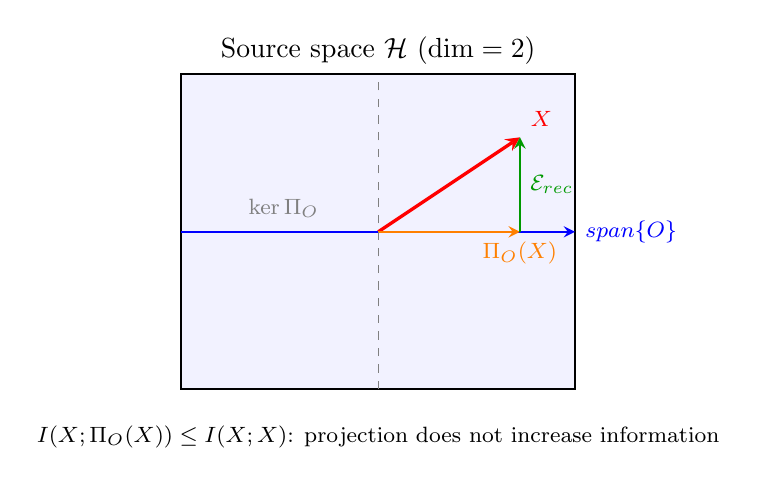
\begin{tikzpicture}[scale=1.0,>=stealth]
  % Source space
  \draw[thick, fill=blue!5] (-2.5,-2) rectangle (2.5,2);
  \node at (0,2.3) {Source space $\mathcal H$ ($\dim=2$)};
  % Source vector
  \draw[->,very thick,red] (0,0) -- (1.8,1.2) node[above right,font=\footnotesize]{$X$};
  % Observer direction
  \draw[->,thick,blue] (-2.5,0) -- (2.5,0) node[right,font=\footnotesize]{$\operatorname{span}\{O\}$};
  % Projection
  \draw[->,thick,orange] (0,0) -- (1.8,0) node[below,font=\footnotesize]{$\Pi_O(X)$};
  % Error
  \draw[->,thick,green!60!black] (1.8,0) -- (1.8,1.2) node[midway,right,font=\footnotesize]{$\mathcal E_{\text{rec}}$};
  % Kernel
  \draw[gray,dashed] (0,-2) -- (0,2);
  \node[gray,font=\footnotesize] at (-1.2,0.3) {$\ker\Pi_O$};
  % Label
  \node[font=\footnotesize] at (0,-2.6) {$I(X;\Pi_O(X))\le I(X;X)$: projection does not increase information};
\end{tikzpicture}
\caption{Projection as information compression: the source vector $X$ decomposes into an observable component $\Pi_O(X)$ and an unobservable component $\mathcal E_{\text{rec}}\in\ker\Pi_O$. The projection discards all the information in the $\ker\Pi_O$ direction.}
\label{fig:projection_information_compression}
\end{figure}

\begin{remark}[Interface with existing information-theoretic frameworks]\label{rem:dyn_projection_info_interface}
The projection information compression of this section connects directly with the following well-established theories:
\begin{enumerate}[label=(\roman*)]
    \item \textbf{Data processing inequality (DPI)}: \cref{thm:dyn_projection_dpi} is the special case of the DPI for deterministic projections. The general form of the DPI is: if $X\to Y\to Z$ is a Markov chain, then $I(X;Y)\ge I(X;Z)$.
    \item \textbf{Rate--distortion theory}: \cref{thm:dyn_projection_rate_distortion} interprets the projection as a zero-rate encoder, whose distortion $D_O$ is the value of the rate--distortion function $R(D)$ at $R=0$.
    \item \textbf{Information loss of PCA}: Geiger and Kubin (2012) proved that the relative information loss of PCA dimensionality reduction is the same as that of direct dimensionality reduction, and that when the rotation matrix is unavailable the loss is infinite. \cref{cor:dyn_projection_kernel_info} of this section gives the explicit form of this conclusion for a single-direction projection.
    \item \textbf{Information bottleneck method}: Chigirev and Bialek (2003) formalised dimensionality reduction as an information bottleneck---the manifold coordinates can acquire only finitely many bits, which naturally determines the optimal dimension. The projection framework of this section may be regarded as the special case of the information bottleneck in the `single-direction' situation.
\end{enumerate}
\end{remark}

\begin{remark}[Scope and open problems]\label{rem:dyn_projection_info_scope}
Prerequisites of the conclusions of this section:
\begin{enumerate}[label=(\roman*)]
    \item $O\neq 0$; when $O=0$ the projection is identically zero and all information is lost;
    \item $X$ is a random vector taking values in $\mathcal H$, with $|X|$ finite almost everywhere;
    \item the existence of the mutual information and of the differential entropy requires the distribution of $X$ to be sufficiently regular (for example absolutely continuous with finite entropy).
\end{enumerate}
The following questions are left open:
\begin{enumerate}[label=(\alph*)]
    \item connecting the upper bound on the mutual information in \cref{thm:dyn_information_compression_bound} quantitatively with the information loss with distance theorem of this chapter (\cref{thm:dyn_information_distance_decay});
    \item the joint information loss of multi-direction projections (observer groups) and the choice of optimal directions;
    \item a quantitative description of the information loss of projection in the quaternion case (a preliminary analysis shows that the dimension of the scalar part drops from $4$ to $1$, so the information loss exceeds that of the complex case).
\end{enumerate}
\end{remark}

\section{Discrete unitary dynamic projection}
\label{sec:dyn_discrete_unitary}

This section discretises the continuous-time evolution of the dynamic epicycle group and establishes the interface with the discrete unitary theory of the `Periodic Manifold' chapter.

\begin{definition}[Time-discretised dynamic epicycle group]\label{def:dyn_discrete_epicycle}
Let the time step be $\Delta t>0$ and $t_m=m\Delta t$ ($m\in\mathbb N$). Let the discrete amplitudes $A_k[m]$, discrete frequencies $\omega_k[m]$ and discrete phases $\phi_k[m]$ satisfy the same regularity as in the continuous case. Define the \textbf{discrete dynamic epicycle group}
\[
\mathcal E_m=\sum_{k=1}^{K}A_k[m]\,e^{i(\omega_k[m]t_m+\phi_k[m])}.
\]
If all the parameters are independent of $m$, it degenerates to the static epicycle group under equally spaced sampling.
\end{definition}

\begin{definition}[Discrete unitary evolution operator]\label{def:dyn_discrete_unitary_operator}
$U_m\in U(N)$ is called a \textbf{discrete unitary evolution operator} if it maps the state $X_m$ at time $t_m$ to the state at time $t_{m+1}$:
\[
X_{m+1}=U_mX_m.
\]
In the case of a dynamic epicycle group, $U_m$ is given by the discrete update rules for the frequencies, amplitudes and phases.
\end{definition}

\begin{proposition}[Modulus-squared conservation under discrete unitary evolution]\label{prop:dyn_discrete_unitary_norm}
If $U_m$ is unitary, then
\[
|X_{m+1}|^2=X_{m+1}^\ast X_{m+1}=X_m^\ast X_m=|X_m|^2.
\]
Hence discrete unitary evolution conserves the modulus squared exactly for any finite step $\Delta t$, independently of $\Delta t\to 0$.
\end{proposition}

\begin{proof}
$X_{m+1}^\ast X_{m+1}=X_m^\ast U_m^\ast U_mX_m=X_m^\ast X_m$.
\end{proof}

\begin{theorem}[Periodicity condition for discrete unitary evolution]\label{thm:dyn_discrete_period_condition}
Let $U$ be a constant unitary operator and $X_{m+1}=UX_m$. Then there exists a positive integer $p$ with $X_{m+p}=X_m$ for all $m$ if and only if $U^p=I$, equivalently all the eigenvalues of $U$ are $p$-th roots of unity.
\end{theorem}

\begin{proof}
$X_{m+p}=U^pX_m$. For any initial value $X_0$ we have $U^pX_0=X_0$ if and only if $U^p=I$. By the spectral theorem for unitary operators, $U^p=I$ is equivalent to all the eigenvalues satisfying $\lambda^p=1$.
\end{proof}

\begin{corollary}[Interface between discrete unitary evolution and Floquet theory]\label{cor:dyn_discrete_floquet}
The eigenvalue $e^{-i\varepsilon}$ of the discrete unitary operator $U$ corresponds to the quasi-energy $\varepsilon$, uniquely determined in the Floquet--Brillouin zone $[-\pi,\pi)$. This agrees completely with \cref{prop:discrete_unitary_floquet} of the `Periodic Manifold' chapter, except that the lattice symbol $n$ used there is replaced by the time index $m$ of this chapter.
\end{corollary}

\begin{proposition}[Continuity condition for discrete dynamic projection]\label{prop:dyn_discrete_projection_continuity}
If the discrete parameters $A_k[m],\omega_k[m],\phi_k[m]$ satisfy a Lipschitz condition in $m$ (that is, $|A_k[m+1]-A_k[m]|\le L\Delta t$ and so on), then as $\Delta t\to 0$ the discrete dynamic projection $\mathcal O_m$ converges uniformly to the continuous dynamic projection $\mathcal O(t)$.
\end{proposition}

\begin{proof}
The difference between the discrete and the continuous dynamic projections is controlled by the triangle inequality: $|\mathcal O_m-\mathcal O(t_m)|\le C(\Delta t)$, where $C$ is given by the Lipschitz constant and a bound on $\mathcal E$.
\end{proof}

\begin{example}[Second-order periodic oscillation]\label{ex:dyn_discrete_c2}
Take $U=-I$; then $X_{m+1}=-X_m$, $|X_m|$ is conserved, and the phase flips by $\pi$ at each step. $p=2$ is the least period. This is the typical instance of a $C_2$ involution in discrete unitary evolution.
\end{example}

\begin{example}[$C_4$ periodic rotation]\label{ex:dyn_discrete_c4}
Take $U=R_{\pi/2}$ (rotation of the plane by $\pi/2$); then $U^4=I$ and $p=4$. This agrees with \cref{ex:lattice_c4} of the `Periodic Manifold' chapter.
\end{example}

\begin{remark}[Relation between discrete unitary and continuous dynamic]\label{rem:dyn_discrete_vs_continuous}
The discrete unitary dynamic projection is the realisation of the continuous dynamic projection under equally spaced sampling. The differences between the two are threefold:
\begin{enumerate}[label=(\roman*)]
    \item in the discrete case the conservation of the modulus squared is exact, whilst in the continuous case it holds in the limiting sense;
    \item the discrete period $p$ and the continuous period $T$ are related by $T=p\Delta t$;
    \item in the discrete case $U$ is allowed to differ at each step (time-varying unitary), in which case the conservation of the modulus squared still holds exactly, but the periodicity condition must be checked segment by segment.
\end{enumerate}
\end{remark}

\section{Scale-dependent sampling theory}
\label{sec:dyn_sampling}

This section systematically establishes scale-dependent sampling theory. The sampling of the source by the observer is controlled by two parameters: the observer scale $\sigma$ and the observation distance $r$. This section gives the rigorous definitions and basic properties of the sampling rate, the number of sampling points, the sampling duration and the sampling orbit. This theory is the foundation of the next section, `information loss with distance'.

\begin{definition}[Scale-dependent sampling rate]\label{def:dyn_sampling_rate}
Let the observer scale be $\sigma>0$, the observation distance $r>0$ and the reference sampling rate $R_0>0$. Define the \textbf{sampling rate}
\[
R(r,\sigma)=R_0\frac{\sigma}{r^2+\sigma}.
\]
$R(r,\sigma)$ denotes the number of samples the observer collects from the source per unit time.
\end{definition}

\begin{definition}[Scale-dependent number of sampling points]\label{def:dyn_sampling_points}
Let the reference number of sampling points be $N_0>0$. Define the \textbf{number of sampling points}
\[
N(r,\sigma)=N_0\frac{\sigma}{r^2+\sigma}.
\]
$N(r,\sigma)$ denotes the total number of samples the observer can collect in a unit duration.
\end{definition}

\begin{definition}[Scale-dependent sampling duration]\label{def:dyn_sampling_duration}
Let the fundamental period of the source be $T_{\text{src}}>0$. Define the \textbf{sampling duration}
\[
T_{\text{samp}}(r,\sigma)=\frac{N(r,\sigma)}{R(r,\sigma)}=\frac{N_0}{R_0},
\]
that is, the sampling duration is independent of both the distance and the observer scale, and is determined solely by the reference parameters $N_0,R_0$.
\end{definition}

\begin{proposition}[Invariance of the sampling duration]\label{prop:dyn_sampling_duration_invariance}
The sampling duration $T_{\text{samp}}$ is independent of both the distance $r$ and the observer scale $\sigma$:
\[
\frac{\partial T_{\text{samp}}}{\partial r}=\frac{\partial T_{\text{samp}}}{\partial\sigma}=0.
\]
Hence the sampling duration is a \textbf{scale invariant}---a fact that contrasts with the distance dependence of the sampling rate and of the number of sampling points.
\end{proposition}

\begin{proof}
By \cref{def:dyn_sampling_duration}, $T_{\text{samp}}=N_0/R_0$ is a constant, so both partial derivatives vanish.
\end{proof}

\begin{definition}[Sampling orbit]\label{def:dyn_sampling_orbit}
Let the continuous trajectory of the source be $X:\mathbb R\to\mathcal H$ and let the sampling step be $\tau(r,\sigma)=1/R(r,\sigma)$. Define the \textbf{sampling orbit} by
\[
\{(t_m,\,X(t_m)):t_m=m\tau(r,\sigma),\;m\in\mathbb Z\}.
\]
The sampling orbit is the sequence of values of the source trajectory at the discrete time points.
\end{definition}

\begin{proposition}[Lattice spacing of the sampling orbit]\label{prop:dyn_sampling_orbit_spacing}
The relation between the sampling step and the distance is
\[
\tau(r,\sigma)=\frac{1}{R(r,\sigma)}=\frac{r^2+\sigma}{R_0\sigma}.
\]
Hence $\tau$ is monotonically increasing in $r$ and monotonically decreasing in $\sigma$:
\[
\frac{\partial\tau}{\partial r}>0,\qquad
\frac{\partial\tau}{\partial\sigma}<0.
\]
That is, the greater the distance, the sparser the sampling points; the larger the observer scale, the denser the sampling points.
\end{proposition}

\begin{proof}
Differentiating directly from \cref{def:dyn_sampling_rate} and \cref{def:dyn_sampling_orbit}: $\tau=(r^2+\sigma)/(R_0\sigma)$, $\partial\tau/\partial r=2r/(R_0\sigma)>0$, $\partial\tau/\partial\sigma=-r^2/(R_0\sigma^2)<0$.
\end{proof}

\begin{theorem}[Resolution of the sampling orbit]\label{thm:dyn_sampling_resolution}
Let the least resolvable period of the source be $T_{\min}$. Then by the sampling theorem, the necessary and sufficient condition for the sampling orbit to resolve $T_{\min}$ is
\[
\tau(r,\sigma)\le T_{\min}/2,
\]
that is,
\[
r^2\le\frac{R_0\sigma T_{\min}}{2}-\sigma=\sigma\left(\frac{R_0T_{\min}}{2}-1\right).
\]
Hence there exists a \textbf{resolution distance} $r_{\text{res}}=\sqrt{\sigma(R_0T_{\min}/2-1)}$; when $r>r_{\text{res}}$, the sampling orbit cannot resolve the least resolvable period of the source.
\end{theorem}

\begin{proof}
By the Nyquist--Shannon sampling theorem, only when the sampling frequency satisfies $R(r,\sigma)\ge 2/T_{\min}$ can the least period $T_{\min}$ be recovered without aliasing. Substituting into \cref{def:dyn_sampling_rate} gives the result.
\end{proof}

\begin{corollary}[Information recoverability of the sampling orbit]\label{cor:dyn_sampling_recoverability}
When $r\le r_{\text{res}}$, the source trajectory can be recovered uniquely from the sampling orbit; when $r>r_{\text{res}}$, the high-frequency components of the source trajectory are aliased and cannot be recovered completely.
\end{corollary}

\begin{proof}
By the Nyquist--Shannon sampling theorem: when the sampling condition is met, complete recovery is possible; when it is not, the high-frequency components are aliased.
\end{proof}

\begin{figure}[htbp]
\centering
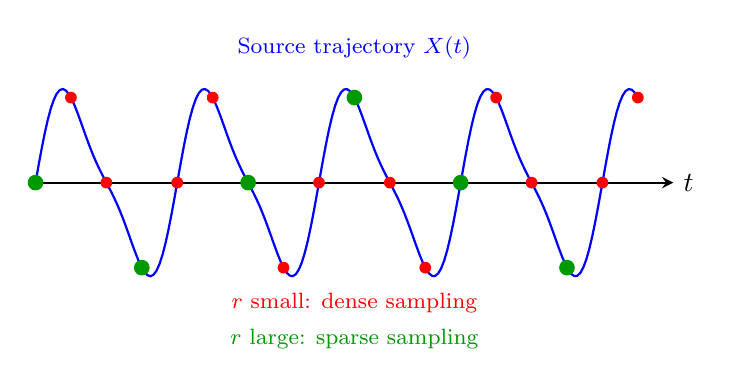
\begin{tikzpicture}[scale=0.9,>=stealth]

  \draw[->, thick] (0,0) -- (9,0) node[right]{$t$};

  \draw[thick, blue, domain=0:8.5, samples=200] plot (\x, {1.2*sin(\x*180)+0.3*sin(\x*360)});
  \node[blue, font=\footnotesize] at (4.5,1.9) {Source trajectory $X(t)$};

  \foreach \x in {0,0.5,1.0,...,8.5} {
    \pgfmathsetmacro{\y}{1.2*sin(\x*180)+0.3*sin(\x*360)}
    \node[circle, fill, red, inner sep=1.5pt] at (\x,\y) {};
  }

  \foreach \x in {0,1.5,3.0,4.5,6.0,7.5} {
    \pgfmathsetmacro{\y}{1.2*sin(\x*180)+0.3*sin(\x*360)}
    \node[circle, fill, green!60!black, inner sep=2pt] at (\x,\y) {};
  }
  \node[red, font=\footnotesize] at (4.5,-1.7) {$r$ small: dense sampling};
  \node[green!60!black, font=\footnotesize] at (4.5,-2.2) {$r$ large: sparse sampling};
\end{tikzpicture}
\caption{Sampling orbit: the greater the distance, the sparser the sampling points. Close-range sampling (red points) can resolve the high-frequency detail of the source, whilst long-range sampling (green points) loses high-frequency information.}
\label{fig:dyn_sampling_orbit}
\end{figure}

\begin{proposition}[Monotonicity of the sampling function]\label{prop:dyn_sampling_monotonicity}
For any $r,\sigma>0$,
\[
\frac{\partial R}{\partial r}<0,\qquad
\frac{\partial N}{\partial r}<0,\qquad
\frac{\partial R}{\partial\sigma}\ge 0,\qquad
\frac{\partial N}{\partial\sigma}\ge 0.
\]
That is, the sampling rate and the number of sampling points decrease strictly with distance and are non-decreasing in the observer scale.
\end{proposition}

\begin{proof}
Differentiating directly from \cref{def:dyn_sampling_rate}: $\partial R/\partial r=-2R_0\sigma r/(r^2+\sigma)^2<0$, $\partial R/\partial\sigma=R_0r^2/(r^2+\sigma)^2>0$. The same holds for $N$.
\end{proof}

\begin{property}[Basic properties of the sampling functions]\label{prop:dyn_sampling_properties}
\begin{enumerate}[label=(\roman*)]
    \item \textbf{Boundedness}: $0<R(r,\sigma)\le R_0$, $0<N(r,\sigma)\le N_0$;
    \item \textbf{Asymptotic behaviour}: $R(r,\sigma)\sim R_0\sigma/r^2$ ($r\to\infty$); $R(0,\sigma)=R_0$, $N(0,\sigma)=N_0$;
    \item \textbf{Scale covariance}: $R(\lambda r,\lambda^2\sigma)=R(r,\sigma)$ ($\lambda>0$).
\end{enumerate}
\end{property}

\begin{proof}
(i) From $\sigma/(r^2+\sigma)\le 1$. (ii) As $r\to\infty$, $r^2+\sigma\sim r^2$, giving the asymptotic formula; at $r=0$, $\sigma/\sigma=1$. (iii) Direct substitution gives the result.
\end{proof}

\begin{remark}[Physical origin of the sampling function]\label{rem:dyn_sampling_physical_source}
The form of the scale-dependent sampling function $R(r,\sigma)=R_0\sigma/(r^2+\sigma)$ comes from the following geometric picture: the source radiates into space and the observer receives at distance $r$. The received signal strength decays as $1/r^2$, whilst the effective receiving area of the observer is proportional to the observer scale $\sigma$. When $r^2\ll\sigma$ the received signal saturates ($R\approx R_0$); when $r^2\gg\sigma$ the received signal decays as $1/r^2$.
\end{remark}

\section{Information loss with distance}
\label{sec:dyn_information_distance}

This section formalises the scale-dependent sampling theory of the previous section as the `information loss with distance' theorem. The core conclusion is that information observability decays asymptotically as $1/r^2$ with distance, and that when the number of sampling points is less than $1$ the source is completely invisible to the observer.

\begin{remark}[Theoretical positioning]\label{rem:dyn_information_distance_positioning}
`Information loss with distance' is not, within the system of this book, independent of existing theories, but a direct corollary of the \textbf{scale-dependent sampling model}: the observer scale $\sigma$ and the observation distance $r$ jointly determine the sampling rate $R(r,\sigma)$ and the number of sampling points $N(r,\sigma)$, both of which decrease monotonically in $r$; when the number of sampling points is less than $1$, the source is completely invisible to the observer. The canonical definition of the model is given in \cref{sec:dyn_sampling}; this section merely restates the conclusions and gives the information-theoretic reading.
\end{remark}

\begin{definition}[Information observability]\label{def:dyn_information_observability}
Define the \textbf{information observability} of the source at distance $r$ by
\[
\mathcal I(r,\sigma)=N(r,\sigma)=N_0\frac{\sigma}{r^2+\sigma}.
\]
$\mathcal I\ge 1$ means that the source is sufficiently sampled, $\mathcal I\in(0,1)$ means that the source is undersampled, and $\mathcal I\to 0$ means that the source is asymptotically invisible.
\end{definition}

\begin{theorem}[Information loss with distance theorem]\label{thm:dyn_information_distance_decay}
Let $r_{\max}(\sigma)=\sqrt{(N_0-1)\sigma}$ (when $N_0>1$). Then
\begin{enumerate}[label=(\roman*)]
    \item sufficient-sampling region: for $r\le r_{\max}$ we have $\mathcal I(r,\sigma)\ge 1$, and the source is observed sufficiently;
    \item undersampling region: for $r>r_{\max}$ we have $\mathcal I(r,\sigma)<1$, and the source is observed only partially;
    \item asymptotic invisibility: as $r\to\infty$, $\mathcal I(r,\sigma)\to 0$;
    \item threshold distance: $\mathcal I(r_{\max},\sigma)=1$, and $\mathcal I<1$ for $r>r_{\max}$.
\end{enumerate}
\end{theorem}

\begin{proof}
By \cref{def:dyn_information_observability}, $\mathcal I=N(r,\sigma)$. The inequality $N(r,\sigma)\ge 1$ is equivalent to $N_0\sigma/(r^2+\sigma)\ge 1$, that is, $r^2\le (N_0-1)\sigma$. Taking $r_{\max}=\sqrt{(N_0-1)\sigma}$ gives (i) and (iv). For $r>r_{\max}$ we have $N<1$, giving (ii). As $r\to\infty$, $N\sim N_0\sigma/r^2\to 0$, giving (iii).
\end{proof}

\begin{corollary}[Asymptotic power law]\label{cor:dyn_information_asymptotic}
When $r\gg\sqrt{\sigma}$,
\[
\mathcal I(r,\sigma)\sim \frac{N_0\sigma}{r^2},
\]
that is, the information observability decays as $1/r^2$. This agrees in form with the intensity decay in free-space optical communication and with the inverse-square laws of the Coulomb and gravitational fields.
\end{corollary}

\begin{proof}
$r^2+\sigma\sim r^2$ (for $r\gg\sqrt\sigma$); substituting gives $\mathcal I\sim N_0\sigma/r^2$.
\end{proof}

\begin{proposition}[Compensation of information observability by the observer scale]\label{prop:dyn_information_sigma_compensation}
For fixed distance $r$, increasing the observer scale $\sigma$ can raise the information observability:
\[
\frac{\partial \mathcal I}{\partial \sigma}\ge 0.
\]
The threshold distance increases monotonically with $\sigma$ according to $r_{\max}(\sigma)=\sqrt{(N_0-1)\sigma}$.
\end{proposition}

\begin{proof}
This follows directly from \cref{prop:dyn_sampling_monotonicity} and \cref{thm:dyn_information_distance_decay}.
\end{proof}

\begin{figure}[htbp]
\centering
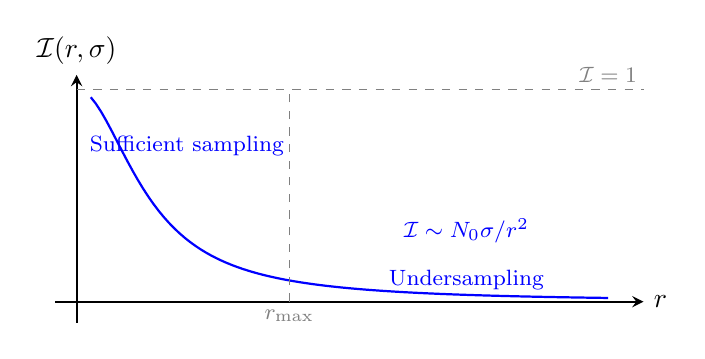
\begin{tikzpicture}[scale=0.9,>=stealth]
  \draw[->, thick] (-0.3,0) -- (8,0) node[right]{$r$};
  \draw[->, thick] (0,-0.3) -- (0,3.2) node[above]{$\mathcal I(r,\sigma)$};

  \draw[thick,blue,domain=0.2:7.5,samples=100] plot (\x,{3.0/(\x*\x+1)});
  \draw[gray,dashed] (0,3.0) -- (8,3.0);
  \node[gray,font=\footnotesize] at (7.5,3.2) {$\mathcal I=1$};
  \draw[gray,dashed] (3.0,0) -- (3.0,3.0);
  \node[gray,font=\footnotesize] at (3.0,-0.2) {$r_{\max}$};
  \node[blue,font=\footnotesize] at (5.5,1.0) {$\mathcal I\sim N_0\sigma/r^2$};
  \node[blue,font=\footnotesize, xshift=0.5cm] at (1.0,2.2) {Sufficient sampling};
  \node[blue,font=\footnotesize] at (5.5,0.3) {Undersampling};
\end{tikzpicture}
\caption{Decay of information observability with distance: for $r\le r_{\max}$ the sampling is sufficient, whilst for $r>r_{\max}$ it decays asymptotically as $1/r^2$.}
\label{fig:info_distance_decay}
\end{figure}

\begin{example}[Numerical example: $\sigma=1$, $N_0=100$]\label{ex:dyn_information_numeric}
Take $\sigma=1$ and $N_0=100$. The threshold distance is $r_{\max}=\sqrt{99}\approx 9.95$.
\begin{itemize}
    \item $r=1$: $N=100\cdot 1/(1+1)=50>1$, sufficient sampling;
    \item $r=10$: $N=100/101\approx 0.99$, marginal undersampling;
    \item $r=100$: $N=100/10001\approx 0.00999$, severe loss;
    \item $r\to\infty$: $\mathcal I\sim 100/r^2\to 0$ (asymptotically invisible).
\end{itemize}
\end{example}

\begin{property}[Basic properties of information observability]\label{prop:dyn_information_properties}
\begin{enumerate}[label=(\roman*)]
    \item \textbf{Monotonicity}: $\mathcal I(r,\sigma)$ is monotonically non-increasing in $r$ and monotonically non-decreasing in $\sigma$;
    \item \textbf{Boundedness}: $\mathcal I(r,\sigma)>0$, and it tends to $0$ as $r\to\infty$;
    \item \textbf{Asymptotic decay}: $\mathcal I(r,\sigma)\sim N_0\sigma/r^2$ ($r\to\infty$);
    \item \textbf{Scale covariance}: $\mathcal I(\lambda r,\lambda^2\sigma)=\mathcal I(r,\sigma)$ ($\lambda>0$).
\end{enumerate}
\end{property}

\begin{proof}
(i)(ii) By \cref{def:dyn_information_observability} and \cref{prop:dyn_sampling_monotonicity}. (iii) By \cref{cor:dyn_information_asymptotic}. (iv) Direct substitution: $N(\lambda r,\lambda^2\sigma)=N_0\lambda^2\sigma/(\lambda^2r^2+\lambda^2\sigma)=N(r,\sigma)$.
\end{proof}

\begin{remark}[Comparison with existing theories]\label{rem:dyn_information_distance_compare}
The `information loss with distance' of this section agrees in form with the following theories, but has a different starting point:
\begin{enumerate}[label=(\roman*)]
    \item \textbf{Shannon information theory}: the channel capacity decays with the signal-to-noise ratio, and the signal-to-noise ratio decays with distance through geometric spreading; this section starts from the number of sampling points.
    \item \textbf{Free-space optical communication}: the received intensity decays as $1/r^2$; the asymptotic power law $N_0\sigma/r^2$ of this section is of the same order.
    \item \textbf{Radar equation}: the two-way return gives $1/r^4$; squaring the one-way model of this section gives exactly this.
    \item \textbf{Sampling theory}: the decline in resolution with distance is an equivalent statement of the decline in sampling rate.
\end{enumerate}
The contribution of this section is to attribute all these phenomena uniformly to the \textbf{joint action of the observer scale and the distance on the sampling rate}, rather than to introduce new physical assumptions.
\end{remark}

\begin{remark}[Scope and open problems]\label{rem:dyn_information_distance_scope}
Prerequisites of the conclusions of this section:
\begin{enumerate}[label=(\roman*)]
    \item the concrete form of the sampling functions $R(r,\sigma)$ and $N(r,\sigma)$ is given by \cref{def:dyn_sampling_rate}; if another decay law is used instead (such as $1/r$ or $1/r^3$), the form of the conclusions is unchanged but the exponent changes;
    \item $\sigma>0$ and $N_0>1$; when $\sigma\to 0$ or $N_0\le 1$ the threshold distance degenerates to zero or becomes negative, and must be discussed separately;
    \item this section discusses only one-way geometric spreading, and does not touch on mechanisms such as multipath, scattering or quantum entanglement.
\end{enumerate}
The following questions are left open:
\begin{enumerate}[label=(\alph*)]
    \item connecting the information observability quantitatively with the DFT leakage estimate of the `Harmonic Analysis' chapter;
    \item the optimal strategy for information recovery under the cooperation of multiple observers;
    \item whether the power law of information loss with distance changes in the quaternion case (a preliminary analysis shows that the conservation of the modulus leaves the exponent unchanged, but that phase information is lost in addition).
\end{enumerate}
\end{remark}

\begin{remark}[Unified logic of this chapter]\label{rem:dyn_unified_logic}
The core logic of this chapter may be summarised in the following three steps:
\begin{enumerate}[label=(\arabic*)]
    \item \textbf{Composition}: the time group $T$ and the space group $S$ are added, giving the composite vector $X=T+S$ (or $q_T+q_S$ in the quaternion case).
    \item \textbf{Projection}: the observer functor $\Pi_O$ projects the composite vector to the observable scalar $\mathcal O=\Pi_O(X)$.
    \item \textbf{Reconstruction}: the reconstruction functor $\Pi_O^\ast$ back-projects the observable scalar to an estimate $\widehat X=\Pi_O^\ast(\mathcal O)$ in the source space. By the adjunction, $\Pi_O\dashv\Pi_O^\ast$, with the counit the identity and the unit not an isomorphism---this formalises the core fact that `observation is information loss'.
\end{enumerate}
The envelope $\varrho=|\mathcal E|$ is the invariant of the composite object under the common phase rotation (\cref{def:dyn_envelope}, \cref{prop:dyn_envelope_sup}): it separates the `fast phase' from the `slow amplitude' and is an intermediate object lying before the projection.

The discrete unitary dynamic projection provides the interface under time discretisation; scale-dependent sampling theory gives the relation between spatial resolution and distance; and information loss with distance is the natural corollary of the two within the observer projection framework.
\end{remark}

\section*{Seven-theme comparison table for this chapter}

\begin{center}
\renewcommand{\arraystretch}{1.3}
\begin{tabular}{@{}p{2.2cm}p{10.5cm}@{}}
\toprule
Theme & Corresponding content in this chapter \\
\midrule
Translation & Dynamic adjustment of the observer vector (\cref{def:dyn_observer}); translation of the rotation angles of the three planes and the three sphere groups (\cref{def:dyn_rotating_planes}, \cref{def:dyn_rotating_quaternion_groups}) \\
Scaling & The weight introduced by the observer modulus (\cref{lem:dyn_triple_weight}); slow amplitude modulation of the envelope (\cref{def:dyn_envelope}, \cref{prop:dyn_envelope_beat}); preservation of the quaternion norm (\cref{prop:dyn_quaternion_rotation_norm}); scale covariance of the sampling functions (\cref{prop:dyn_sampling_properties}) \\
Rotation & Independent rotation of the three planes (\cref{def:dyn_rotating_planes}); independent rotation of the three sphere groups (\cref{def:dyn_rotating_quaternion_groups}); non-commutative quaternion rotation (\cref{thm:dyn_quaternion_noncommutative}) \\
Balance & Linearity of the projection (\cref{prop:dyn_projection_linearity}); additivity of synthesis--projection (\cref{prop:dyn_triple_additivity}); scale invariance of the sampling duration (\cref{prop:dyn_sampling_duration_invariance}) \\
Symmetry & Symmetry of the projection (\cref{prop:dyn_projection_symmetry}); symmetry of the quaternion inner product (\cref{lem:dyn_quaternion_inner_symmetry}); commutativity under the additive convention (\cref{cor:dyn_quaternion_additive_commutative}) \\
Closure & Invariance under synchronous rotation of the three planes (\cref{thm:dyn_sync_invariance}); invariance under synchronous rotation of the three sphere groups (\cref{thm:dyn_quaternion_sync_invariance}); adjunction closure of the observer functor (\cref{thm:dyn_observer_adjunction}) \\
Period & Instantaneous frequency of the dynamic projection (\cref{thm:dyn_projection_continuity}); single-frequency frequency shift (\cref{cor:dyn_doppler}); three-group beat frequency (\cref{cor:dyn_triple_beat}); envelope period and modulation order (\cref{thm:dyn_envelope_difference}, \cref{prop:dyn_modulation_order}); discrete periodicity condition (\cref{thm:dyn_discrete_period_condition}); resolution of the sampling orbit (\cref{thm:dyn_sampling_resolution}) \\
\bottomrule
\end{tabular}
\end{center}

\section*{Exercises}

\begin{enumerate}[leftmargin=3em, label=\textbf{Exercise \arabic*}]
    \item According to Definition \ref{def:dyn_epicycle} and Definition \ref{def:dyn_epicycle_group_def},
    explain how an epicycle $\gamma_{A,\omega,\phi}(t)=Ae^{i(\omega t+\phi)}$
    corresponds to a simple complex function, and how an epicycle group is a finite sum of simple complex functions.
    Using the epicycle group with $K=3$,
    \[
    \mathcal{E}(t)=A_1e^{i(\omega_1 t+\phi_1)}+A_2e^{i(\omega_2 t+\phi_2)}+A_3e^{i(\omega_3 t+\phi_3)}
    \]
    write out its corresponding period series form, and indicate which level of parameter the amplitude, the phase and the frequency correspond to respectively.

    \item Prove Proposition \ref{prop:dyn_epicycle_period_condition}:
    the epicycle group $\mathcal{E}(t)=\sum_{k=1}^K A_k e^{i(\omega_k t+\phi_k)}$ ($A_k>0$)
    is a periodic function if and only if all the $\omega_k$ generate a discrete subgroup,
    that is, $\omega_k/\omega_0\in\mathbb{Z}$ for all $k$, where $\omega_0=\gcd\{\omega_k\ne0\}$.
    Prove sufficiency and necessity separately, and state that the least positive period is $2\pi/\lvert\omega_0\rvert$ (an integer fraction of it when $\omega_0\notin\Omega$); when all $\omega_k=0$ there is no least positive period.

    \item Prove Proposition \ref{prop:dyn_epicycle_ball_norm}:
    the orbit of the episphere $\beta_{a,\mathbf{u},\theta}(t)=ae^{\mathbf{u}\theta t}$
    lies on the three-dimensional sphere of radius $a$, $S^3_a=\{q\in\mathbb{H}:|q|=a\}$.
    Complete the proof using $e^{\mathbf{u}\theta t}=\cos(\theta t)+\mathbf{u}\sin(\theta t)$
    and $|\mathbf{u}|=1$.

    \item Verify Remark \ref{rem:dyn_epicycle_ball_noncommutative}:
    if the rotation axes of two epispheres differ ($\mathbf{u}_1\neq\mathbf{u}_2$), then
    \[
    e^{\mathbf{u}_1\theta_1 t}e^{\mathbf{u}_2\theta_2 t}
    \neq e^{\mathbf{u}_2\theta_2 t}e^{\mathbf{u}_1\theta_1 t}.
    \]
    Taking $\mathbf{u}_1=i$, $\mathbf{u}_2=j$ and $\theta_1=\theta_2=1$,
    verify this non-commutativity by explicit computation using $ij=k$ and $ji=-k$.

    \item Prove Proposition \ref{prop:dyn_projection_linearity} and Proposition \ref{prop:dyn_projection_symmetry}:
    \begin{enumerate}[label=(\roman*)]
        \item the projection is real-linear in $\mathcal{E}$:
              $\mathcal{O}[\alpha\mathcal{E}_1+\beta\mathcal{E}_2]
              =\alpha\mathcal{O}[\mathcal{E}_1]+\beta\mathcal{O}[\mathcal{E}_2]$;
        \item the projection is symmetric:
              $\mathcal{O}(t)=\operatorname{Re}[\mathcal{E}(t)\overline{u(t)}]
              =\operatorname{Re}[u(t)\overline{\mathcal{E}(t)}]$.
    \end{enumerate}

    \item Prove Lemma \ref{lem:dyn_single_freq}:
    taking $\mathcal{E}(t)=Ae^{i\omega t}$ and observer $u(t)=e^{i\omega_0 t}$, we have
    \[
    \mathcal{O}(t)=A\cos((\omega-\omega_0)t).
    \]
    Also prove Corollary \ref{cor:dyn_doppler}: the frequency seen by the observer is
    $\omega_{\text{obs}}=\omega-\omega_0$,
    and when $\omega_0=\omega$ the observation result is the constant $A$.

    \item Prove Theorem \ref{thm:dyn_projection_continuity}:
    if $A_k,\omega_k,\phi_k,\theta$ are all $C^1$ functions,
    then the observation result $\mathcal{O}(t)$ is a $C^1$ function.
    Furthermore, if $|\mathcal{E}(t)|\neq0$, the instantaneous frequency of $\mathcal{O}(t)$ is
    \[
    \Omega_{\mathcal{O}}(t)=\frac{d}{dt}\arg(\mathcal{E}(t)\overline{u(t)}),
    \]
    and verify that it degenerates to $\omega-\omega_0$ in the single-frequency case.

    \item Prove Proposition \ref{prop:dyn_triple_additivity}:
    the observation result is additive with respect to the time group and the space group:
    \[
    \mathcal{O}(t)=\operatorname{Re}[T(t)\overline{O(t)}]
    +\operatorname{Re}[S(t)\overline{O(t)}].
    \]
    Also prove Lemma \ref{lem:dyn_triple_weight}:
    in the general case
    \[
    \mathcal{O}(t)=\operatorname{Re}[(T(t)+S(t))\overline{\widehat{O}(t)}]\cdot|O(t)|,
    \qquad
    \widehat{O}(t)=O(t)/|O(t)|.
    \]

    \item Verify the beat-frequency formula of Corollary \ref{cor:dyn_triple_beat}:
    taking $T(t)=Ae^{i\omega t}$, $S(t)=Be^{i\nu t}$ and $O(t)=Ce^{i\mu t}$,
    we have
    \[
    \mathcal{O}(t)=AC\cos((\omega-\mu)t)+BC\cos((\nu-\mu)t).
    \]
    Using the concrete values $A=1,B=1,C=1,\omega=10,\nu=12,\mu=11$,
    compute $\mathcal{O}(t)$ and find the beat period.

    \item Prove Proposition \ref{prop:dyn_rotation_phase_shift}:
    the rotating three planes are equivalent to applying phase shifts to $T_0,S_0,O_0$ respectively before composition,
    that is,
    \[
    \mathcal{O}(t)=\operatorname{Re}\big[(T_0e^{i(\theta_T-\theta_O)}
    +S_0e^{i(\theta_S-\theta_O)})\overline{O_0}\big].
    \]
    Explain why only the two relative rotation angles $\theta_T-\theta_O$ and $\theta_S-\theta_O$ take effect.

    \item Prove Theorem \ref{thm:dyn_sync_invariance}:
    if $\theta_T(t)=\theta_S(t)=\theta_O(t)=\theta(t)$,
    then the observation result is the same as in the static case:
    \[
    \mathcal{O}(t)=\operatorname{Re}[(T_0(t)+S_0(t))\overline{O_0(t)}].
    \]
    Also write out the frequency-shift formula under asynchronous rotation (Corollary \ref{cor:dyn_async_beat}).

    \item Prove Proposition \ref{prop:dyn_quaternion_projection_types}:
    the scalar part of the quaternion inner product $\operatorname{Re}[q\overline{p}]$
    and the conjugation action $p^{-1}qp$ are two different kinds of projection:
    \begin{enumerate}[label=(\roman*)]
        \item $\operatorname{Re}[q\overline{p}]$ is the inner-product projection on $\mathbb{R}^4$, and outputs a real number;
        \item $p^{-1}qp$ is a rotation of $SO(3)$, and outputs a quaternion.
    \end{enumerate}
    Taking $q=\mathbf{i}$ and $p=\mathbf{j}$, compute the two projections explicitly.

    \item Prove Theorem \ref{thm:dyn_quaternion_noncommutative}:
    consider the additive synthesis $X_+=q_T+q_S$ and the multiplicative synthesis $X_\times=q_Tq_S$;
    then in general
    \[
    \operatorname{Re}[X_+\overline{q_O}]\neq\operatorname{Re}[X_\times\overline{q_O}],
    \]
    and $q_Tq_S\neq q_Sq_T$.
    Taking $q_T=\mathbf{i}$, $q_S=\mathbf{j}$ and $q_O=\mathbf{k}$, verify this explicitly.

    \item Prove Theorem \ref{thm:dyn_quaternion_sync_invariance}:
    if $r_T=r_S=r_O=r$, then
    \[
    \mathcal{Q}(t)=\operatorname{Re}[(q_{T,0}(t)+q_{S,0}(t))\overline{q_{O,0}(t)}].
    \]
    Complete the proof using Lemma \ref{lem:dyn_quaternion_conjugation_scalar}:
    $\operatorname{Re}[rxr^{-1}]=\operatorname{Re}[x]$.

    \item Prove Theorem \ref{thm:dyn_unified_representation}:
    all five models of this chapter can be written as special cases of the unified observer operator
    \[
    \Pi_O(X)=\operatorname{Re}[X\overline{O}]
    \]
    Compare item by item with Definition \ref{def:dyn_projection}, \ref{def:dyn_triple_projection},
    \ref{def:dyn_rotating_planes_projection}, \ref{def:dyn_quaternion_projection},
    \ref{def:dyn_rotating_quaternion_projection},
    and write out the $X$ and the $O$ of each model.

    \item Verify the four axioms of the projection operator in Corollary \ref{cor:dyn_projection_axioms}:
    real linearity, observer sign reversal, non-expansiveness and zero-observer degeneracy.
    Complete the proof using the bilinearity of the inner product and the Cauchy--Schwarz inequality.

    \item Prove Theorem \ref{thm:dyn_observer_adjunction}:
    the observer functor $\Pi_O$ and the reconstruction functor $\Pi_O^\ast$ form an adjoint pair
    $\Pi_O\dashv\Pi_O^\ast$,
    that is,
    \[
    \langle\Pi_O(X),y\rangle_{\mathcal{H}_{\text{obs}}}
    =\langle X,\Pi_O^\ast(y)\rangle_{\mathcal{H}}.
    \]
    Compute both sides and verify that they are equal, and explain why the unit $\eta$ is not an isomorphism.

    \item Prove Theorem \ref{thm:dyn_projection_dpi} (the data processing inequality):
    let $X\to Y=\Pi_O(X)\to Z=\Pi_O^\ast(Y)$ be a Markov chain;
    then $I(X;Y)\ge I(X;Z)$.
    Explain the meaning of the statement that projection does not increase information,
    and point out the contribution of the unobservable subspace to the information loss
    in Corollary \ref{cor:dyn_projection_kernel_info}.

    \item Verify Example \ref{ex:dyn_uniform_projection}:
    let $X=e^{i\Theta}$ with $\Theta$ uniformly distributed on $[0,2\pi)$, and let
    $O=e^{i\theta_0}$. Then $\Pi_O(X)=\cos(\Theta-\theta_0)$
    follows the Arcsine distribution, and the information loss is $\log 4$.
    Compute $h(\Pi_O(X))$ and $h(X)$, and verify that their difference equals $\log 4$.

    \item Prove Theorem \ref{thm:dyn_discrete_period_condition}:
    let $U$ be a constant unitary operator and $X_{m+1}=UX_m$.
    Then there exists a positive integer $p$ with $X_{m+p}=X_m$ for all $m$
    if and only if $U^p=I$, equivalently all the eigenvalues of $U$ are $p$-th roots of unity.
    Complete the proof using the spectral theorem for unitary operators,
    and point out its relation to Floquet theory (Corollary \ref{cor:dyn_discrete_floquet}).

    \item Prove Proposition \ref{prop:dyn_sampling_duration_invariance}:
    the sampling duration
    \[
    T_{\text{samp}}(r,\sigma)=\frac{N(r,\sigma)}{R(r,\sigma)}=\frac{N_0}{R_0}
    \]
    is independent of both the distance $r$ and the observer scale $\sigma$.
    Complete the proof using Definition \ref{def:dyn_sampling_rate} and \ref{def:dyn_sampling_points},
    and explain why the sampling rate and the number of sampling points decrease strictly with distance (Proposition \ref{prop:dyn_sampling_monotonicity}).

    \item Prove Theorem \ref{thm:dyn_sampling_resolution}:
    let the least resolvable period of the source be $T_{\min}$;
    then the necessary and sufficient condition for the sampling orbit to resolve $T_{\min}$ is
    \[
    \tau(r,\sigma)\le T_{\min}/2,
    \]
    that is,
    \[
    r^2\le\sigma\left(\frac{R_0 T_{\min}}{2}-1\right).
    \]
    Complete the proof using the Nyquist--Shannon sampling theorem,
    and give the expression for the resolution distance $r_{\text{res}}$.

    \item Prove Theorem \ref{thm:dyn_information_distance_decay}:
    let the threshold distance be $r_{\max}(\sigma)=\sqrt{(N_0-1)\sigma}$;
    then the information observability
    \[
    \mathcal{I}(r,\sigma)=N_0\frac{\sigma}{r^2+\sigma}
    \]
    satisfies:
    \begin{enumerate}[label=(\roman*)]
        \item $\mathcal{I}\ge1$ for $r\le r_{\max}$ (sufficient sampling);
        \item $\mathcal{I}<1$ for $r>r_{\max}$ (undersampling);
        \item $\mathcal{I}\to0$ as $r\to\infty$ (asymptotically invisible).
    \end{enumerate}
    Also prove Corollary \ref{cor:dyn_information_asymptotic}:
    when $r\gg\sqrt{\sigma}$, $\mathcal{I}(r,\sigma)\sim N_0\sigma/r^2$.

    \item Synthesis problem: combining the dynamic epicycle group (Definition \ref{def:dyn_epicycle_group}),
    the rotating three planes (Definition \ref{def:dyn_rotating_planes}),
    the rotating three-sphere groups (Definition \ref{def:dyn_rotating_quaternion_groups})
    and the unified observer operator (Definition \ref{def:dyn_unified_operator}),
    explain how the `compose first, then project' convention of this chapter remains consistent across the five models.
    Point out separately, for each model:
    \begin{enumerate}[label=(\roman*)]
        \item what the composite vector $X$ is;
        \item what the observer $O$ is;
        \item what observation result the projection $\Pi_O(X)=\operatorname{Re}[X\overline{O}]$ gives;
        \item how the reconstruction functor $\Pi_O^\ast$ back-projects from the observation result.
    \end{enumerate}

    \item Prove the difference-frequency expansion of Theorem \ref{thm:dyn_envelope_difference},
    and for $K=3$, $\omega_k=k\omega_0$, $A_k=1$, $\phi_k=0$ compute the least positive period $T_{\text{env}}$ of the envelope $\varrho$,
    showing that it equals the carrier period $2\pi/\omega_0$.
    Then, for the two-component case $\omega_1=\omega_0$, $\omega_2=2\omega_0$, compute the modulation order $N$
    and use Proposition \ref{prop:dyn_modulation_order} to verify that the least positive period of the composite signal is $T_{\text{env}}$.
\end{enumerate}

